\documentclass[12pt,a4paper,header]{abnt}

\usepackage[brazil]{babel}        
\usepackage[utf8]{inputenc} 

\usepackage{hyperref}
\usepackage{breakurl}
\usepackage{bookmark}
\usepackage{amsmath,amssymb,amsfonts,undertilde}
\usepackage{graphicx}
\usepackage{subfigure}
\usepackage{fancyhdr}
\usepackage{siunitx}
\usepackage{longtable}
\usepackage{booktabs}

\usepackage[svgnames]{xcolor}
\usepackage{listings}

%%%%%%%%%%%%%%%%%%%%%%%%%%%
%Teoremas, definicoes, etc%
%%%%%%%%%%%%%%%%%%%%%%%%%%%

\newtheorem{thm}{Teorema}[section]
\newtheorem{cor}[thm]{Corolário}
\newtheorem{lem}[thm]{Lema}
\newtheorem{defi}[thm]{Definição}
\newtheorem{exe}[thm]{Exemplo}
\newtheorem{prop}[thm]{Proposição}

\renewcommand{\ABNTchapterfont}{\bfseries}
\renewcommand{\ABNTsectionfont}{\bfseries}

\fancypagestyle{logouff}{%
	\renewcommand{\headrulewidth}{0pt}
	\fancyhead{}
	\fancyhead[R]{
\includegraphics[width=0.7\textwidth]{logoUFF.pdf}}% Your logo/image
  	\setlength{\headheight}{30pt} 
  	\setlength{\headsep}{2cm}
}


\begin{document}

%%%%%%%%%%%%%%%%%%%%%%%%%%%%%%
%colocar aqui o nome do aluno%
%%%%%%%%%%%%%%%%%%%%%%%%%%%%%%
\autor{Leonardo Filgueira}


%%%%%%%%%%%%%%%%%%%%%%%%%%%%%%%%%%%%%
%colocar aqui o título da monografia%
%%%%%%%%%%%%%%%%%%%%%%%%%%%%%%%%%%%%%
\titulo{Sistemas de recomendação usando o software R}


%%%%%%%%%%%%%%%%%%%%%%%%%%%%%%%%%%%
%colocar aqui o nome do orientador%
%%%%%%%%%%%%%%%%%%%%%%%%%%%%%%%%%%%
\orientador{Luciane Ferreira Alcoforado}  


%%%%%%%%%%%%%%%%%%%%%%%%%%%%%%%%%%%%%%%%%%%%%%%%%%%
%colocar aqui o nome do co-orientador, caso exista%
%%%%%%%%%%%%%%%%%%%%%%%%%%%%%%%%%%%%%%%%%%%%%%%%%%%
\coorientador{Rodrigo Otávio de Araújo Ribeiro}


%%%%%%%%%%%%%%%%%%%%%%%%%%%%%%%%%%%%%%%%%%%%%%%%%%%
%colocar aqui a data da apresentacao da monografia%
%%%%%%%%%%%%%%%%%%%%%%%%%%%%%%%%%%%%%%%%%%%%%%%%%%%
\data{14 de dezembro de 2018}



%%%%%%%%%%%%%%%%%%%%%%%%%%%
%nao mexer até a linha 180%
%%%%%%%%%%%%%%%%%%%%%%%%%%%


\comentario{Monografia apresentada para obtenção do grau de Bacharel em Estatística pela Universidade Federal Fluminense.}

\instituicao{Departamento de Estatística \par Instituto de Matemática e Estatística \par Universidade Federal Fluminense}

\local{Niterói - RJ, Brasil}

\capa

\vspace{10cm}


%folha de rosto
%--------------

\begin{titlepage}

\thispagestyle{logouff}

\vspace{2cm}

\hspace{.2\textwidth} % posicionando a minipage
\begin{minipage}{.7\textwidth}

\begin{flushright}

{\large \bf \ABNTautordata} \\[3cm]

{\Large \bf \ABNTtitulodata}\\[3cm]

{\bf Trabalho de Conclusão de Curso}\\[1cm]

\end{flushright}

\begin{espacosimples}

\ABNTcomentariodata

\end{espacosimples}

\vspace{1cm}

\hfill Orientador: Prof. \ABNTorientadordata

\end{minipage}

\vspace{7cm}

\begin{center}

\ABNTlocaldata

\ABNTdatadata

\end{center}

\end{titlepage}


% ficha catalografica
%-------------------
\newpage
\null
\vfill

% \begin{left}
\fbox{

\includegraphics[scale=1]{ficha_catalografica.PNG}
}
% \end{center}
\vspace{1cm}

%folha de aprovacao com as assinaturas - Editar os membros da banca
%------------------------------------------------------------------
\begin{folhadeaprovacao}

\thispagestyle{logouff}

\hspace{.2\textwidth} % posicionando a minipage
\begin{minipage}{.7\textwidth}

\begin{flushright}

{\large \bf \ABNTautordata}\\[1cm]

{\large \bf \ABNTtitulodata}\\[1cm]

\end{flushright}

Monografia de Projeto Final de Graduação sob o título \textit{``\ABNTtitulodata''},
defendida por \ABNTautordata~e aprovada em \ABNTdatadata, na cidade de Niterói,
no Estado do Rio de Janeiro, pela banca examinadora constituída pelos
professores:

\begin{flushright}

\begin{espacosimples}

%assinatura

%%%%%%%%%%%%%%%%%%%%%%%%%%%%%%%%%%%%%%%%%
%Preencher os dados dos membros da banca%
%%%%%%%%%%%%%%%%%%%%%%%%%%%%%%%%%%%%%%%%%

\vspace{2cm}
\noindent\rule{8cm}{0.4pt}\\
{\bf Profa. Dra. Luciane Ferreira Alcoforado}\\
Departamento de Estatística -- UFF\\


\vspace{2cm}
\noindent\rule{8cm}{0.4pt}\\
{\bf Prof. Dr. Steven Dutt Ross}\\
UNIRIO\\


\vspace{2cm}
\noindent\rule{8cm}{0.4pt}\\
{\bf Prof. Dr. Rodrigo Otávio de Araújo Ribeiro}\\
UERJ\\

\end{espacosimples}

\end{flushright}

\vspace{2cm}
\hfill Niterói, \ABNTdatadata

\end{minipage}


%\vfill \hfill Niterói, \ABNTdatadata \hspace{1cm} 

\end{folhadeaprovacao}

%%%%%%%%%%%%%%%%%%%%%%%%%%%%%%%%%%%%%%%
%escreva aqui o resumo do seu trabalho%
%%%%%%%%%%%%%%%%%%%%%%%%%%%%%%%%%%%%%%%
\begin{resumo}

O trabalho apresenta algumas técnicas utilizadas na realização de sistemas de recomendação e realiza um estudo de caso, ao utilizar uma base de dados de avaliações de filmes por usuários. É aplicada sobre essa base uma técnica de filtragem colaborativa a fim obter recomendações de filmes aos usuários. Informações como gêneros dos filmes, avaliação dos usuários e número de filmes avaliados serão utilizadas de forma a agrupar os usuários em clusters, utilizando as técnicas de particionamento CLARA e K-means, de forma a aplicar a filtragem colaborativa para cada um dos clusters, em separado. Realiza-se uma comparação de acurácia dos modelos, fazendo a divisão em base de treino (para construir o modelo) e base de teste (para verificar a acurácia), além de uma verificação do tempo de execução, com o objetivo de verificar se, nas condições desse estudo, a clusterização torna a recomendação mais acurada.

\vspace{1cm}
\noindent Palavras-chaves:
Sistemas de recomendação, filtragem colaborativa, clusterização.

\end{resumo}

% %%%%%%%%%%%%%%%%%%%%%%%%%%%%%%%%
% %escreva aqui a sua dedicatória% (opcional)
% %%%%%%%%%%%%%%%%%%%%%%%%%%%%%%%%
% \chapter*{Dedicatória}
% % Aqui entra a sua dedicatória. 
% 
% 
% 
%%%%%%%%%%%%%%%%%%%%%%%%%%%%%%%%%%
%escreva aqui seus agradecimentos% (opcional)
%%%%%%%%%%%%%%%%%%%%%%%%%%%%%%%%%%
\chapter*{Agradecimentos}

Agradeço a Deus por ter me permitido caminhar até aqui. Aos meus pais por terem sempre se preocupado em me dar uma boa educação, mesmo com todas as dificuldades. Também aos meus avós, que sempre se preocuparam com meu crescimento, em muitos aspectos, e foram muito importantes durante todo o tempo. A alguns amigos, na universidade, no estágio ou na Igreja, me incentivaram a prosseguir neste tempo e não os menciono aqui para não ser injusto com quem minha memória falhar. Também à equipe do projeto ``Estatística é com R!", que me fez crescer durante boa parte de graduação, à minha orientadora, que acreditou em confiou em minha capacidade, além dos professores da banca, que me ajudaram a melhorar alguns pontos do trabalho, com críticas bem colocadas. À todas as pessoas que, diretamente ou indiretamente contribuíram para minha formação (não só a graduação), meu muito obrigado!



\tableofcontents{}
\listoffigures
\listoftables

\chapter{Introdução} \label{cap:introducao}

A partir do aumento de informação disponível com a popularização da Internet e com a possibilidade de armazená-las, surge o desafio de lidar com este grande conjunto de dados\cite{isinkaye2015recommendation}. Este aumento de informações desafia o site (loja, rede social, streaming de vídeo/músicas) que recebe todos os dados dos usuários que visitam o endereço, mas também pode se tornar um problema para o usuário que, diante da grande quantidade de produtos disponíveis para compra, pode levar muito tempo para achar o produto desejado\cite{mild2002collaborative}.

Sistemas de recomendação podem ser definidos como técnicas de \textit{machine learning} (aprendizado de máquina) que filtram um grande conjunto de dados, tendo como base informações dos usuários e itens\cite{takahashi2015estudo}. A partir dessas técnicas são indicados item(ns) aos usuários. De maneira mais simples, sistemas de recomendação são técnicas que fornecem sugestões de itens, de forma que os usuários possam tomar melhores decisões\cite{gorakala2015building}, a depender do contexto onde a recomendação se aplica.

Os sistemas de recomendação têm como objetivo recomendar itens que interessariam aos usuários\cite{melville2011recommender}, beneficiando o usuário e a loja, pois eles aumentam o desempenho da loja, fazendo-a vender uma quantidade maior de produtos, e também facilitam a procura do usuário fazendo-o achar o(s) produto(s) desejado(s) em um menor tempo\cite{isinkaye2015recommendation}. 

O primeiro sistema de recomendação foi criado na década de $90$ e tinha como nome ``filtragem colaborativa'', pois o sistema funcionava com base na colaboração entre os grupos de pessoas interessados. Contudo, o termo ``sistemas de recomendação'' é mais usado por ser mais geral, não sendo realizada, necessariamente, nenhuma colaboração entre pessoas\cite{reategui2005sistemas}. Um dos primeiros a ser utilizado, ainda no início dos anos $1990$, tinha como objetivo recomendar documentos eletrônicos num sistema de e-mail desenvolvido pela \textit{Xerox}\cite{goldberg1992using}. Já em 1996 o \textit{Yahoo} utilizou sistemas de recomendação em uma de suas páginas, aplicando em larga escala\cite{reategui2005sistemas}, coisa que hoje é feita comumente por diversos sites e serviços.

É facilmente perceptível no cotidiano o uso de sistemas de recomendação em ambientes on-line. Ao usar a \textit{Netflix}, sugestões para o usuário são oferecidas, baseadas nas atrações já assistidas e/ou avaliadas. Sites de compras como a \textit{Amazon} também oferecem sugestões de produtos ao usuário baseado em visitas à página dos produtos ou no comportamento de outros usuários que compraram um mesmo produto. Também em redes sociais, como no \textit{YouTube}, são sugeridos vídeos baseados no histórico do internauta e nas suas avaliações, ou então no \textit{Facebook}, que recomenda lista de pessoas que o usuário pode conhecer\cite{gorakala2015building}.

Uma forma de comunicar ao usuário a recomendação processada é por meio do e-mail marketing, que é um canal de comunicação direto com o cliente\cite{takahashi2015estudo}. Após a pessoa aceitar receber tais mensagens, pode-se utilizar dessa comunicação direta para enviar ao usuário os itens para ele recomendados. Assim, podem-se aplicar recomendações também no meio físico, bastando cadastrar os clientes e utilizar o e-mail marketing.

Sistemas de recomendação podem utilizar como informação a avaliação (\textit{rating}) dada pelos usuários aos itens, podendo a avaliação estar expressa de diferentes maneiras\cite{shapira2011recommender}:

\begin{itemize}

\item Avaliações numéricas: O usuário avalia um item numa escala numérica, como no site da \textit{Amazon}, onde o usuário dá uma nota de até 5 estrelas.

\item Avaliações qualitativas: A avaliação é dada por frases definidas, como: "Concordo totalmente", "Concordo parcialmente", ...

\item Avaliações binárias: O usuário seleciona se gostou ou não gostou do item, como a \textit{Netflix}, atualmente, recebe as avaliações.

\item Avaliação unária: A indicação se refere a se o usuário visualizou, comprou ou então avaliou o item positivamente.

\end{itemize}

Esses tipos de avaliação são um tipo de \textit{input} para um sistema de recomendação, chamado de \textit{explicit feedback}, o que significa que o usuário explicitamente informou seu interesse a respeito do item. Contudo, essa informação nem sempre está disponível, como é o caso de lojas físicas, que não recebem uma nota do usuário aos produtos comprados. Nesses casos, existe a necessidade de  utilizar técnicas que buscam de alguma forma inferir os ratings, o \textit{implicit feedback}\cite{oard1998implicit}.  Existem algumas maneiras de se obter este feedback implícito, como histórico de compras ou padrões de busca (ambientes on-line)\cite{hu2008collaborative}.

\section{Técnicas de recomendação}

Existem diferentes categorias de sistemas de recomendação, que podem ser classificados em: Filtragem baseada em conteúdo (\textit{Content-based filtering}), filtragem colaborativa (\textit{Collaborative filtering}) e sistemas de recomendação híbridos (\textit{Hybrid Recommender Systems})\cite{melville2011recommender}, que aplicam as duas primeiras filtragens separadamente ou num único modelo que une as duas abordagens\cite{takahashi2015estudo}, aproveitando suas vantagens e buscando eliminar suas desvantagens\cite{shapira2011recommender}.

\subsection{Filtragem baseada em conteúdo}

Os sistemas nesta categoria recomendam itens similares aos que o usuário gostou no passado\cite{gorakala2015building}. Para isto é necessário utilizar informações das características de um produto\cite{shapira2011recommender} e comparar com o perfil do usuário, de acordo com itens já conhecidos pelo usuário. Considerando filmes como itens, se um usuário avaliou positivamente filmes do gênero de ação, então o sistema recomendará a este usuário filmes de ação. Por outro lado, a filtragem baseada em conteúdo não leva em conta a similaridade de preferência entre os usuários, mas apenas o histórico do usuário e as características dos itens\cite{gorakala2015building}.

Algumas das técnicas utilizadas neste tipo de filtragem são: TF/IDF (\textit{Term Frequency Inverse Document}), \textit{naive Bayes Classifier}, árvores de decisão ou redes neurais\cite{isinkaye2015recommendation}. 

\subsection{Filtragem colaborativa}

Na filtragem colaborativa são recomendados itens de acordo com as avaliações de todos os usuários\cite{melville2011recommender}. Existem duas maneiras principais de realizar essa filtragem: baseado em memória ou em modelo\cite{dakhel2011new}. Nos algoritmos baseados em memória, verifica-se a similaridade entre usuários ou entre itens (vizinhança), de acordo com suas avaliações passadas. Essa técnica é a mais utilizada para realizar recomendações\cite{shapira2011recommender}. Um exemplo simples seria: Se o usuário 1 comprou o item A, B e C, e o usuário 2 comprou os itens A e C, então recomenda-se o item B para o usuário 2.

Os algoritmos de filtragem colaborativa utilizam uma matriz, chamada de matriz de avaliações (\textit{ratings matrix}), usualmente representada como na tabela \ref{rating_matrix}.

\begin{table}[h]
\caption{Típica matriz \textbf{R} de avaliações}
\label{rating_matrix}
\centering
\begin{tabular}{@{}c|cccc@{}}
\cmidrule(l){2-5}
\textbf{}   & Item 1       & Item 2       & $\cdots$ & Item m       \\ \midrule
Usuário 1   & $r_{(1, 1)}$ &              & $\cdots$ &              \\
Usuário 2   &              & $r_{(2, 2)}$ & $\cdots$ & $r_{(2, m)}$ \\
$\vdots$    & $\vdots$     & $\vdots$     & $\ddots$ & $\vdots$     \\
Usuário $n$ &              &              & $\cdots$ & $r_{(n, m)}$ \\ \bottomrule
\end{tabular}
\end{table}

Onde $r_{(i, j)}$ é a avaliação (\textit{rating}) do usuário $i$ dado ao item $j$. Em geral, os usuários não tiveram contato com todos os itens, então os itens não recebem avaliações de todos os usuários, produzindo então uma matriz esparsa (com grande quantidade de valores faltantes). Os algoritmos buscam, então, preencher a matriz de avaliações com previsões para os valores faltantes.

À medida, porém, que os números de usuários e items aumentam, podem surgir problemas ao realizar a filtragem, como o aumento do tempo necessário, além de recursos computacionais, para executar o algoritmo, chamado de problema de escalabilidade\cite{dakhel2011new}. Além disso, existe o problema da esparsidade, pois um usuário, em geral, não avaliou uma grande quantidade de itens, mas apenas uma pequena quantidade, o que pode causar a impossibilidade do cálculo de medidas de similaridade (pois itens precisam ter sido avaliados por dois usuários), ou então pode levar, pela pequena quantidade de informação utilizada no cálculo da medida, a uma medida que não represente bem a real similaridade entre os usuários\cite{dakhel2011new}.

Buscando reduzir o tempo de processamento e melhores medidas de acurácia podem ser utilizados métodos de agrupamento (cluster)\cite{o1999clustering}. Uma possibilidade é agrupar usuários, de acordo com alguma informação disponível em $k$ clusters e, para cada um dos grupos de usuários, aplicar a técnica de recomendação.  

\chapter{Objetivos}

Este trabalho tem os seguintes objetivos:

\section{Objetivo geral}

Realizar um estudo de caso a partir de uma base de avaliação de filmes, de forma a avaliar a acurácia das recomendações utilizando filtragem colaborativa para todo o conjunto de dados e as recomendações utilizando filtragem colaborativa para cada cluster de usuários.

\section{Objetivos específicos}

\begin{itemize}

\item{Descrever informações de filmes e usuários.}
\item{Verificar a proporção de filmes avaliados por gênero.}
\item{Descrever a esparsidade da matriz de avaliações.}
\item{Analisar filmes avaliados e recomendados para determinado usuário.}
\item{Comparar o tempo de execução da recomendação para as configurações escolhidas.}

\end{itemize}

\chapter{Materiais e Métodos}

\section{Conjunto de dados}

Será utilizado um \textit{dataset} disponível no site \textit{grouplens}, disponível em \burl{https://grouplens.org/datasets/movielens/1m/}. O conjunto de dados possui $\num{1000209}$ avaliações de $3900$ filmes dados por $6040$ usuários\cite{harper2016movielens}, que se cadastraram no site \textit{MovieLens} no ano de 2000. De acordo com o próprio site, pessoas podem se inscrever para avaliar filmes e receber recomendações de filmes para assistir.

Os usuários são representados pelo seu ID, que varia entre $1$ e $6040$ e os filmes possuem ID entre $1$ e $3952$. As avaliações têm formato numérico, de até 5 estrelas, com estrelas completas, tendo cada usuário avaliado ao menos 20 filmes.

A base de dados será dividida em duas, treino e teste, na proporção de $70\%$ dos dados para treinar o modelo (base de treino) e $30\%$ da base que será usada para testar o modelo (base de teste). Assim, as notas dadas pelos usuários pertencentes à base de teste serão utilizadas para comparar com as notas previstas pelo modelo.

Será utilizada uma segunda base, que apresenta informações sobre os filmes, como o código, nome e gêneros do filme. Um mesmo filme pode ter sido associado a mais de um gênero, mas nenhum filme não foi associado a algum dos $18$ gêneros existentes.

Executar a tarefa de recomendação é dificultada a medida em que o tamanho da base de dados aumenta, e fazê-la sem utilizar um servidor, com uma quantidade maior de memória e processamento exige que não se utilize uma base maior. Devido a essa limitação, utilizou-se a base escolhida. 

\section{Metodologia}

Na filtragem colaborativa, foco deste trabalho, haverão um conjunto de usuários $U = \{u_1, u_2, \ldots, u_n\}$ e um conjunto de itens $I = \{i_1, i_2, \ldots, i_m \}$, assim como as notas dos usuários aos itens, que serão armazenadas na matriz $\boldsymbol{R}_{n \times m}$ de avaliações\cite{hahsler2015recommenderlab}. Logo, cada linha da matriz $\boldsymbol{R}$ representa um usuário e cada coluna, um item. Os algoritmos utilizados nesse trabalho buscarão preencher os valores faltantes desta matriz, com valores na mesma escala das avaliações presentes na matriz\cite{takahashi2015estudo}. Para executar a filtragem colaborativa será utilizado o algoritmo baseado no usuário.

\subsection{Filtragem colaborativa baseada no usuário (user-based)}

Este algoritmo assume que usuários com preferência similar no passado terão preferências similares no futuro. Então os \textit{ratings} não observados serão previstos a partir das avaliações de uma vizinhança e usuários com gostos similares\cite{hahsler2015recommenderlab}. São então encontrados os vizinhos mais próximos de um usuário ou então todos os usuários que tenham pelo menos uma dada similaridade. O coeficiente de correlação de Pearson pode ser utilizado como medida de similaridade entre dois usuários $a$ e $u$, definida da seguinte maneira\cite{melville2011recommender}:

\begin{equation}
w_{a, u} = \frac{\sum_{i \in I}{(r_{a, i} - \overline{r}_a ) ( r_{u, i} - \overline{r}_u )}}{\sqrt{\sum_{i \in I}{(r_{a, i} - \overline{r}_a )^2} \sum_{i \in I}{(r_{u, i} - \overline{r}_u )^2}}}
\end{equation}

Sendo $I$ o conjunto de itens avaliados pelos dois usuários, $r_{u, i}$ o rating dado pelo usuário $u$ ao item $i$ e $\overline{r}_u$ o rating médio do usuário $u$ a todos os itens por ele avaliados. Em filtragem colaborativa, esse coeficiente é muito usado\cite{su2009survey} e atinge melhores resultados\cite{breese1998empirical}. Por esses motivos, a correlação de Pearson será utilizada como medida de similaridade.

Uma outra maneira de calcular a similaridade entre dois usuários é considerar os ratings de dois usuários como vetores num espaço $m$-dimensional, para, assim, encontrar o cosseno do ângulo entre estes vetores\cite{melville2011recommender}:

\begin{equation}
w_{a, u} = \cos({\vec{r}_a, \vec{r}_u}) = \frac{\vec{r}_a \boldsymbol{\cdot} \vec{r}_u}{\lVert \vec{r}_a\rVert \times \lVert \vec{r}_u\rVert} = \frac{\sum_{i=1}^{m}{r_{a, i} r_{u, i}}}{\sqrt{\sum_{i=1}^{m}{r^2_{a, i}} \sum{_{i=1}^{m}{r^2_{u, i}}}}}
\end{equation}

Por fim, a predição da nota dada ao item $i$ pelo usuário $a$ é dada por:

\begin{equation}
p_{a, i} = \overline{r}_a + \frac{\sum_{u \in V}{(r_{u, i} - \overline{r}_u) w_{a, u}}}{\sum_{u \in V}{\left|w_{a, u}\right|}}
\end{equation}

Sendo $V$ a vizinhança do usuário $a$.

De modo a agrupar os usuários para, então aplicar a filtragem colaborativa, foram utilizadas duas técnicas de particionamento: \textit{CLARA} e \textit{K-means}, descritos a seguir.

\subsection{\textit{CLARA} (Clustering Large Applications)}

Essa técnica foi proposta em 1990, de forma a aplicar a técnica \textit{PAM} (Partitioning Around Medoids), utilizando amostragem para a aplicação da técnica\cite{park2009simple}. O método, então, seleciona aleatoriamente uma parte da base de dados e aplica o algoritmo PAM nesta amostra. 

O algoritmo de agrupamento PAM é baseado na definição de \textit{medoide}, que é o ponto com menor distância, em média, de todos os outros elementos do cluster. O algoritmo, para obter $k$ clusters, é executado da seguinte maneira\cite{do2005agrupamentos}:

\begin{enumerate}

\item{Definir aleatoriamente $k$ medoides.}
\item{Associar cada um dos elementos restantes ao cluster de medoide mais próximo.}
\item{Calcular a dissimilaridade entre um elemento $x_i$ e todos os outros do cluster, e a dissimilaridade entre o medoide e os outros elementos do cluster.}
\item{Caso a distância considerando $x_i$ como novo medoide seja menor que a distância do medoide atual, passe a considerar $x_i$ como medoide daquele cluster.}
\item{Repetir os passos 2 a 4 até não haver troca de medoides.}

\end{enumerate}

Uma desvantagem do PAM é a ineficiência ao ser aplicado para um grande conjunto de dados\cite{park2009simple}. Essa é a razão pela qual foi escolhida a técnica CLARA.

O algoritmo que executa a técnica CLARA segue calculando a função de custo, que é uma média da similaridade entre os medoides e os outros elementos da base\cite{bhat2014k}. A função de custo é definida da seguinte maneira:

\begin{equation}
C(m, D) = \frac{\sum_{i=1}^{n}{d(x_i, cl(m, x_i))}}{n}
\end{equation}

Onde:

\begin{itemize}

\item{$m$ são os medoides encontrados.}
\item{$cl(m,  x_i)$ é o medoide mais próximo de um ponto $x_i$.}
\item{$d(x_i, cl(m, x_i))$ é uma medida de similaridade entre $x_i$ e seu medoide mais próximo.}
\item{$n$ é o número de observações na base de dados $D$.}

\end{itemize}

Todo o processo é repetido um número determinado de vezes e o resultado que obtiver menor função de custo é definido então como o melhor e é retornado\cite{bhat2014k}.

\subsection{\textit{K-Means}}
K-means é uma técnica que particiona elementos em $k$ clusters utilizando-se de centroides, que são os elementos representativos de cada cluster. Este método busca minimizar a soma das distâncias dos elementos de um mesmo cluster. Dados então, uma matriz $D$, de dimensão $m \times n$, e um número de clusters $k$, o algoritmo, então, procede da seguinte maneira\cite{han2011data}:

\begin{enumerate}

\item{São escolhidos, aleatoriamente, $k$ objetos de $D$ como sendo os centroides.}
\item{Cada elemento $D_{i,}$ é associado ao centroide mais próximo, de acordo com a medida de distância adotada (neste caso, a distância Euclidiana).}
\item{Os centroides de cada um dos clusters são calculados.}
\item{Repetir os passos 2 e 3 até que não haja mudanças.}

\end{enumerate}

\subsection{Informações utilizadas para agrupamento}

Com o intuito de agrupar os usuários em clusters, foram utilizadas duas bases de dados: a avaliação média dos usuários para cada categoria e a proporção de filmes assistidos pelos usuários para cada categoria. No primeiro caso, utilizando o rating médio, houveram casos em que alguns gêneros não receberam nenhuma nota, gerando um dado faltante. Para preencher os valores faltantes foi usada a média de notas por categoria.

Para que tivessem sido geradas algumas possibilidades de resultados utilizando clusterização, os usuários foram agrupados desde em 2 clusters até em 15 grupos para cada algoritmo e para cada base: Rating médio e proporção de filmes assistidos por categoria.

\subsection{Medidas de erro}

Para verificar a acurácia do sistema de recomendação, dado que a base utilizada foi dividida em base de treino e de teste, serão comparadas a avaliação prevista e a avaliação observada. Considerando $r_{i,j}$ a avaliação observada e $p_{i,j}$ a avaliação prevista pelo modelo do usuário $i$ ao item $j$, as medidas utilizadas serão\cite{gorakala2015building}:

\subsubsection{Erro médio absoluto}

O erro médio absoluto (EMA) se dá pela soma do módulo das diferenças. 

\begin{equation}
EMA = \frac{1}{nm} \sum_{i=1}^{n} \sum_{j=1}^m \left| r_{i,j} - p_{i,j}  \right|
\end{equation}

\subsubsection{Erro quadrático médio}

O erro quadrático médio (EQM) é a soma das diferenças ao quadrado. Por este motivo, a unidade de medida muda, e a sua interpretação deve ser cautelosa.

\begin{equation}
EQM = \frac{1}{nm} \sum_{i=1}^{n} \sum_{j=1}^m \left( r_{i,j} - p_{i,j}  \right)^2
\end{equation}

\subsubsection{Raiz do erro quadrático médio}

Ao calcular a raiz do EQM obtém-se um número na mesma unidade de medida dos dados.

\begin{equation}
REQM = \sqrt{\frac{1}{nm} \sum_{i=1}^{n} \sum_{j=1}^m \left( r_{i,j} - p_{i,j}  \right)^2}
\end{equation}

\subsection{Software utilizado}

A fim de executar todo o processo de leitura e descrição da base, clusterização, recomendação e avaliação dos resultados, foi utilizada a linguagem de programação R\cite{R}, por meio do ambiente de desenvolvimento RStudio\cite{RStudio}. O pacote do R \textit{recommenderlab}\cite{recommenderlab} executa a recomendação e sua avaliação, produzindo as medidas de erro.

\chapter{Análise dos Resultados}

A matriz de avaliações obtida possui $\num{1000209}$ elementos preenchidos. Desta maneira é possível verificar que aproximadamente $4.68\%$ da matriz possui avaliações. Como uma matriz esparsa, nota-se que a maior parte dos elementos da matriz não possui valores.

Os $6040$ usuários avaliaram pelo menos $20$ filmes. Na figura \ref{hist_num_ratings}, é possível notar que a maior parte dos usuários avaliou até $500$ filmes. Além disso, nota-se que essa distribuição apresenta uma assimetria a direita.

\begin{figure}[h]
\centering
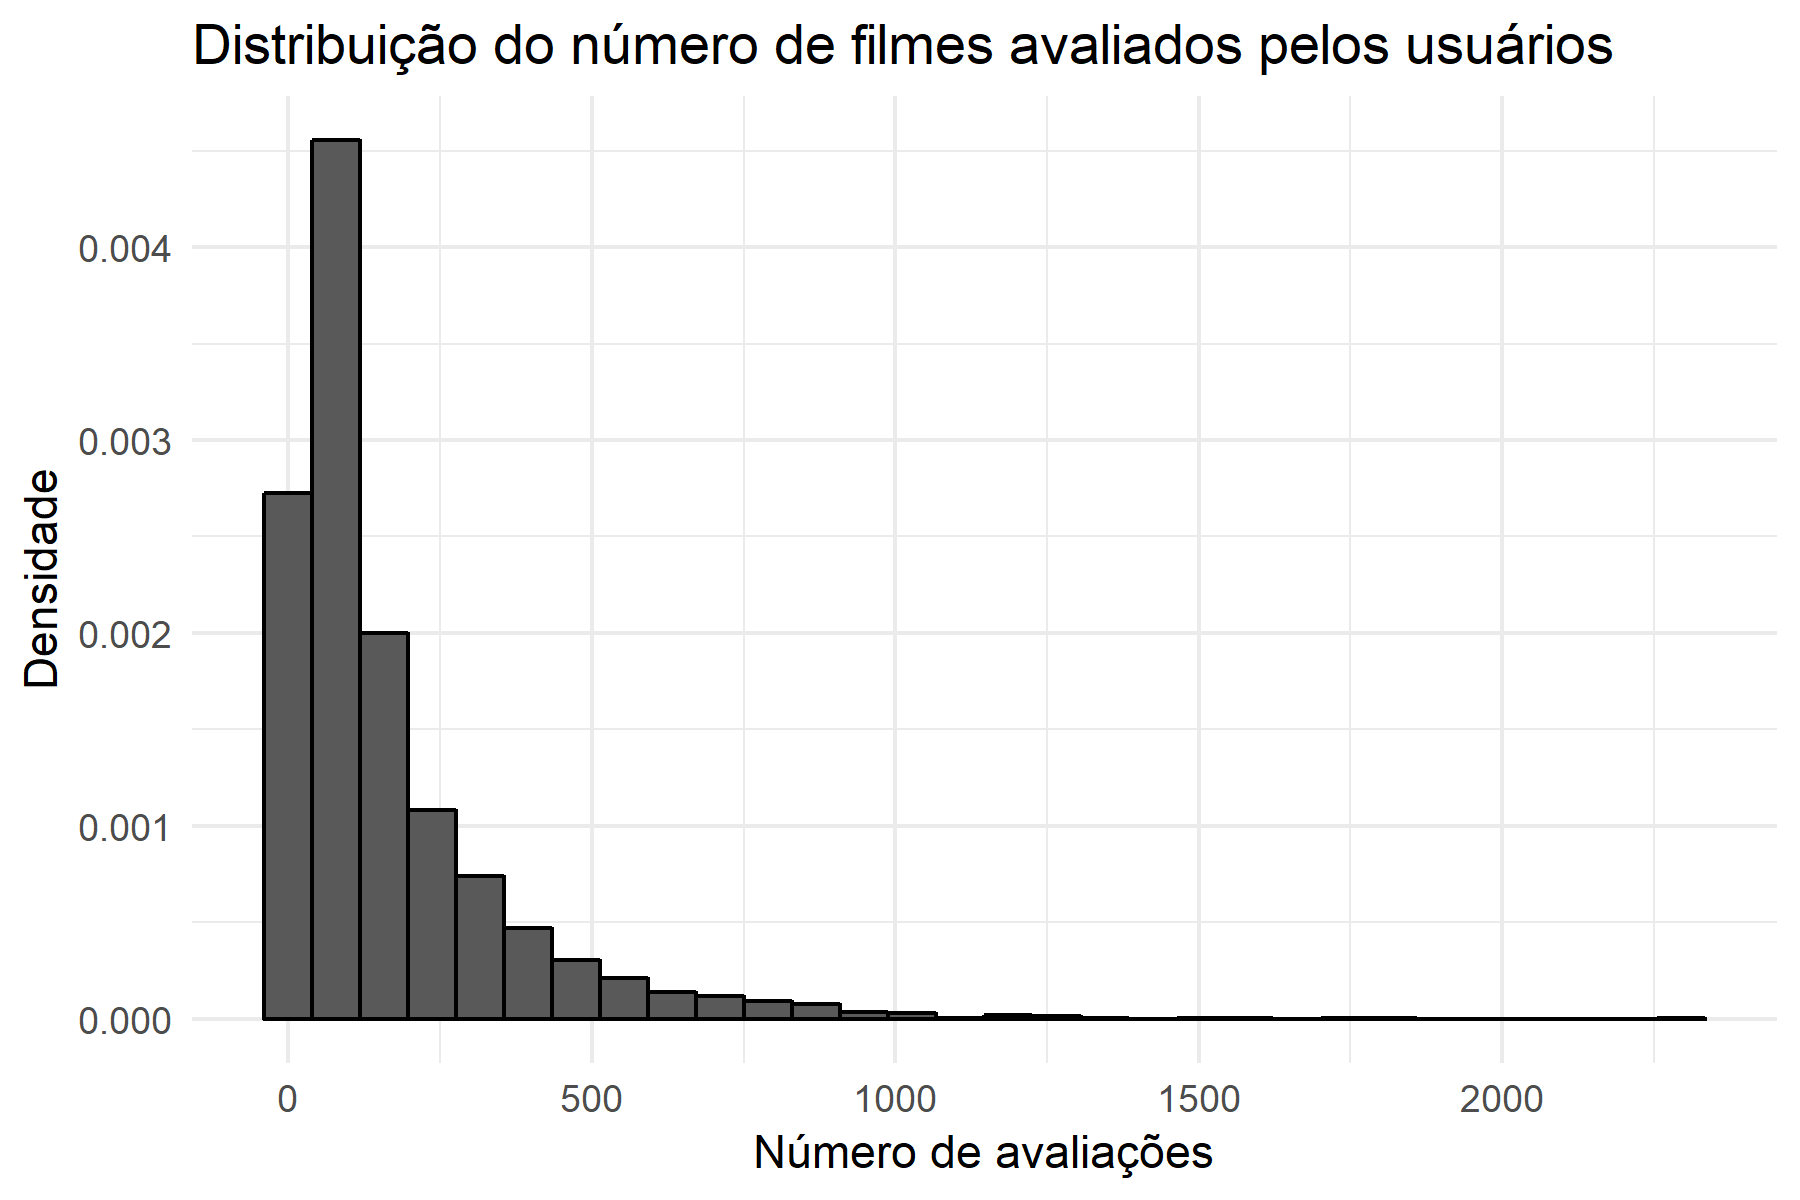
\includegraphics[]{../R/img/Distribuicao_ratings.png}
\caption{Número de filmes avaliados pelos usuários}
\label{hist_num_ratings}
\end{figure}

A tabela \ref{resumo_rating} apresenta algumas medidas resumo a respeito da quantidade de filmes avaliados pelos usuários. Nota-se uma grande amplitude, variância, desvio padrão e coeficiente de variação, o que indica uma grande variabilidade na quantidade de filmes avaliados. Metade dos usuários avaliou até $96$ filmes. Além disso, $75\%$ dos usuários avaliaram até $208$ filmes, o que indica, como já foi indicado na figura \ref{hist_num_ratings}, que um número pequeno de usuários, diferentemente do comportamento da maior parte, avaliou uma grande quantidade de filmes.

\begin{table}[h]
\caption{Medidas resumo da quantidade de filmes avaliados por usuários}
\label{resumo_rating}
\centering
\begin{tabular}{@{}ccccccc@{}}
\toprule
\textbf{Min.} & \textbf{Mediana} & \textbf{Média} & \textbf{Max.} & \textbf{Variância} & \textbf{Desvio padrão} & \textbf{Coef. de variação} \\ \midrule
20            & 96               & 165.6          & 2314          & 37151              & 193                    & 1.16                       \\ \bottomrule
\end{tabular}
\end{table}

A seguir, a tabela \ref{top20_filmes} apresenta os 20 filmes com maior número de avaliações recebidas. Destaca-se a trilogia original de \textit{Star Wars}, cujos filmes receberam, entre si, uma quantidade muito próxima de avaliações dos usuários.

\begin{table}[h]
\caption{Os 20 filmes com mais avaliações recebidas}
\label{top20_filmes}
\begin{tabular}{@{}lc@{}}
\toprule
\textbf{Filme}                                                 & \textbf{Número de avaliações} \\ \midrule
American Beauty (1999)                                & 3428    \\
Star Wars: Episode IV - A New Hope (1977)             & 2991    \\
Star Wars: Episode V - The Empire Strikes Back (1980) & 2990    \\
Star Wars: Episode VI - Return of the Jedi (1983)     & 2883    \\
Jurassic Park (1993)                                  & 2672    \\
Saving Private Ryan (1998)                            & 2653    \\
Terminator 2: Judgment Day (1991)                     & 2649    \\
Matrix, The (1999)                                    & 2590    \\
Back to the Future (1985)                             & 2583    \\
Silence of the Lambs, The (1991)                      & 2578    \\
Men in Black (1997)                                   & 2538    \\
Raiders of the Lost Ark (1981)                        & 2514    \\
Fargo (1996)                                          & 2513    \\
Sixth Sense, The (1999)                               & 2459    \\
Braveheart (1995)                                     & 2443    \\
Shakespeare in Love (1998)                            & 2369    \\
Princess Bride, The (1987)                            & 2318    \\
Schindler's List (1993)                               & 2304    \\
L.A. Confidential (1997)                              & 2288    \\
Groundhog Day (1993)                                  & 2278    \\ \bottomrule
\end{tabular}
\end{table}

A distribuição da quantidade de avaliações recebidas pelos filmes na base de dados é apresentada na figura \ref{filmes_ratings}. $114$ filmes receberam apenas uma avaliação, $50\%$ dos filmes receberam $124$ \textit{ratings} e um filme recebeu $2858$ avaliações de usuários. A variabilidade de ratings recebidos pelos filmes é alta, com um coeficiente de variação igual a $1.42$.

\begin{figure}[h]
\centering
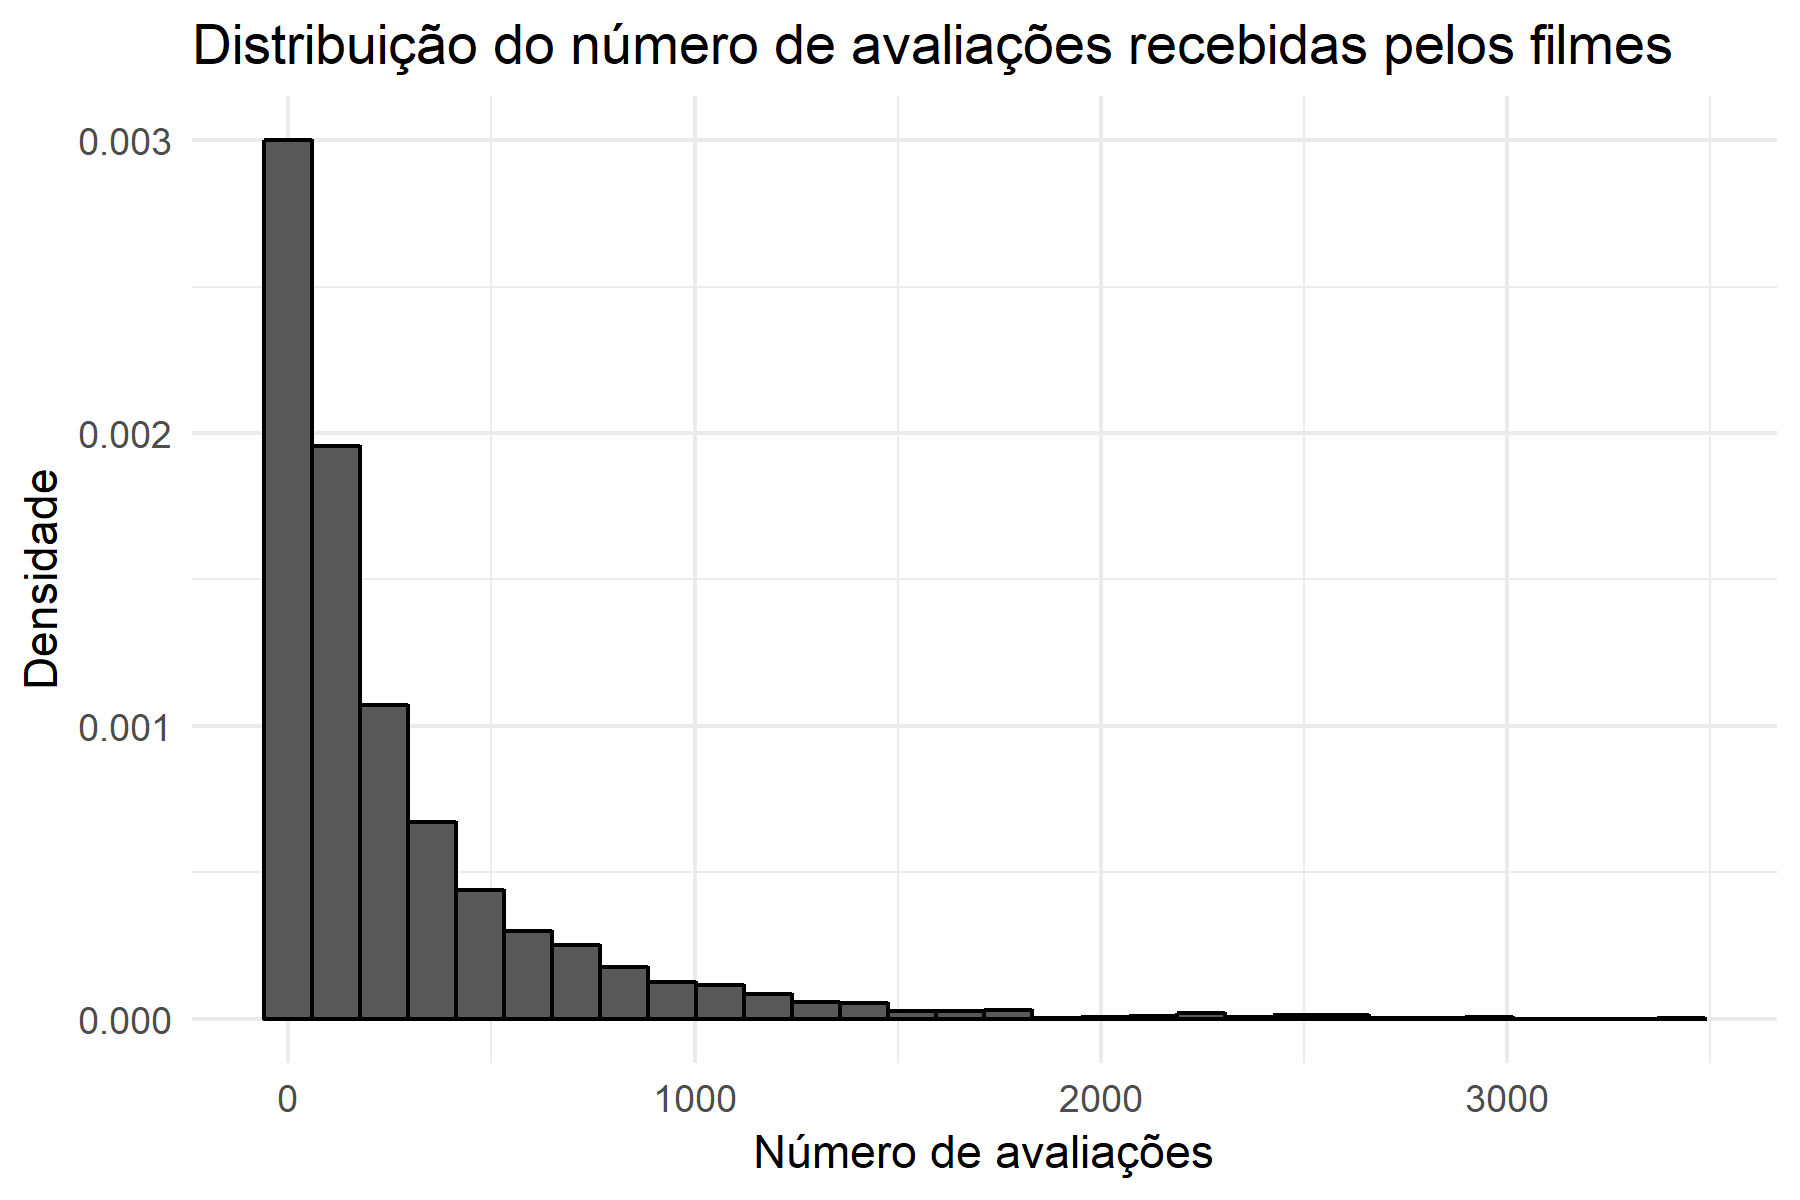
\includegraphics[]{../R/img/ratings_filmes.png}
\caption{Número de avaliações recebidas pelos filmes}
\label{filmes_ratings}
\end{figure}

A tabela \ref{generos} apresenta a quantidade de filmes aos quais cada gênero foi atribuído e a proporção de usuários que avaliaram cada gênero. Como cada filme pode ter sido descrito com mais de um gênero, a soma das frequências é maior que o número de filmes. Nota-se que os gêneros aos quais mais filmes foram associados são drama e comédia. O terceiro gênero com mais filmes associados, ação, apresenta menos de metade do número de filmes, em relação aos dois primeiros. Além desses três gêneros, aventura, romance, thriller, sci-fi e guerra possuem uma proporção acima de $95\%$ de usuários que os avaliaram.

\begin{table}[!htb]
\caption{Gêneros existentes na base e número de filmes associados}
\label{generos}
\centering
\begin{tabular}{@{}lll@{}}
\\
\toprule
\textbf{Gênero} & \textbf{Número de filmes} & \textbf{Proporção de usuários} \\ \midrule
Action & 503 & 0.9954 \\
Adventure & 283 & 0.9758 \\
Animation & 105 & 0.796 \\
Children's & 251 & 0.8747 \\
Comedy & 1200 & 0.9985 \\
Crime & 211 & 0.9374 \\
Documentary & 127 & 0.3714 \\
Drama & 1603 & 0.9995 \\
Fantasy & 68 & 0.803 \\
Film-Noir & 44 & 0.6871 \\
Horror & 343 & 0.8775 \\
Musical & 114 & 0.7871 \\
Mystery & 106 & 0.8498 \\
Romance & 471 & 0.9869 \\
Sci-Fi & 276 & 0.9786 \\
Thriller & 492 & 0.9916 \\
War & 143 & 0.9551 \\
Western & 68 & 0.6788 \\ \bottomrule
\end{tabular}
\end{table}

A figura \ref{genero_rating_medio} apresenta as distribuições de nota média recebida para os gêneros presentes na base. A mediana das avaliações médias encontra-se entre $3$ e $4$ estrelas, com apenas os gêneros \textit{War} (guerra), \textit{Film-Noir} (uma espécie de filme policial) e \textit{Documentary} (documentário) atingindo uma mediana igual a $4$. As medianas mais baixas encontram-se em \textit{Horror} e \textit{Sci-Fi} (Ficção científica), com $3.38$ e $3.58$ como medianas, respectivamente.

\begin{figure}[h]
\centering
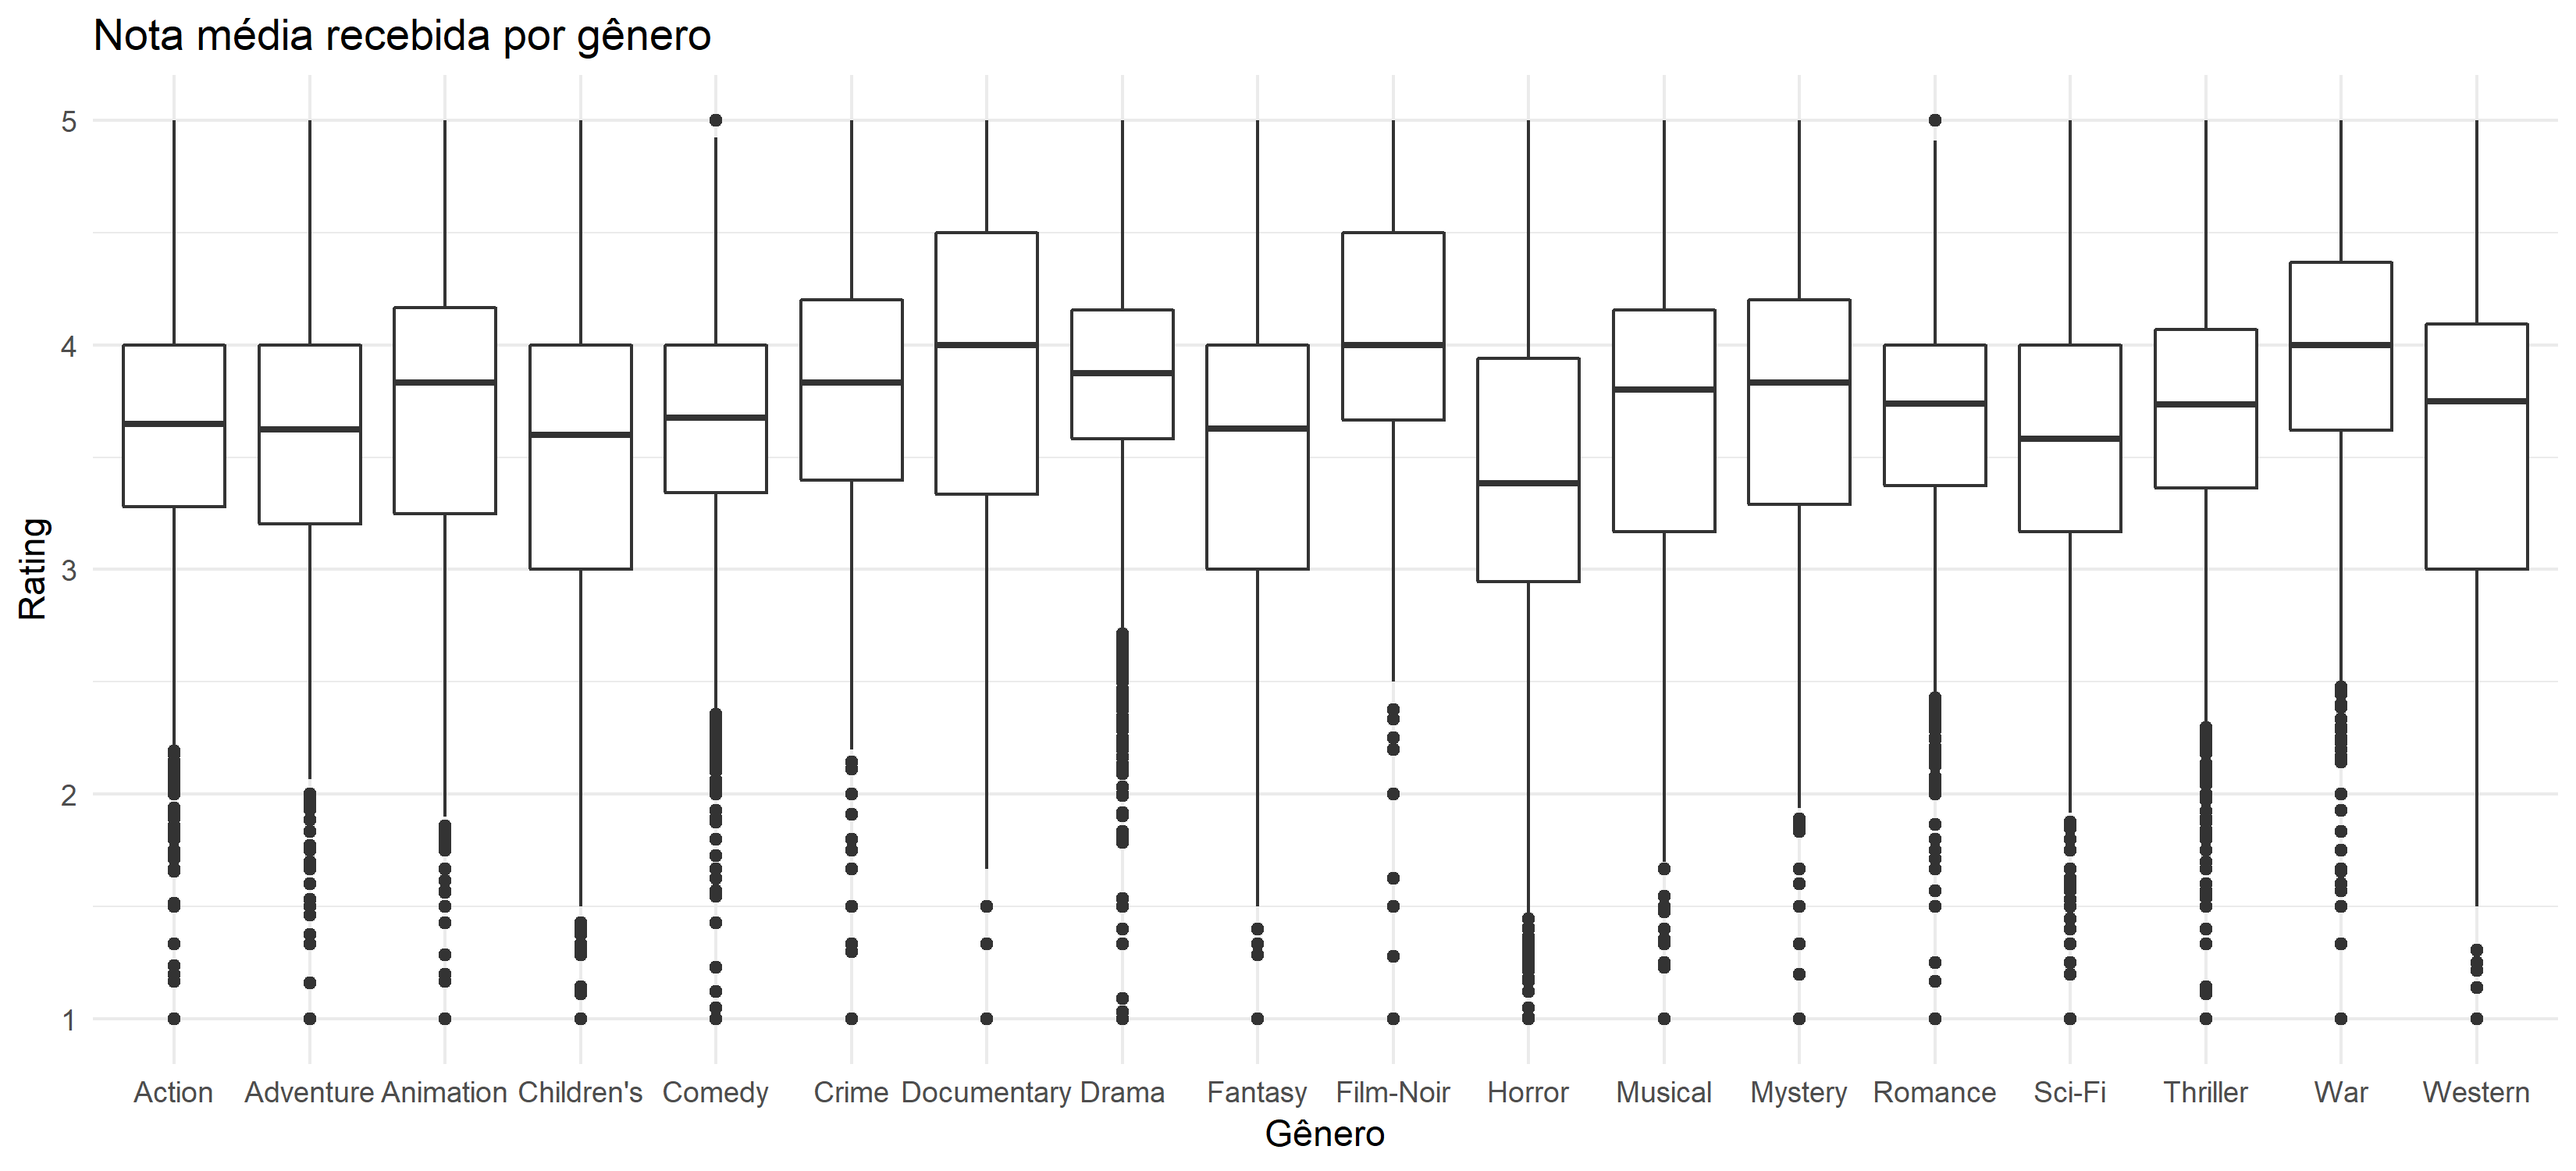
\includegraphics[scale = 0.6]{../R/img/rating_medio_genero.png}
\caption{Distribuição da avaliação médio por gênero}
\label{genero_rating_medio}
\end{figure}

A seguir será verificada a recomendação para um usuário em específico, que avaliou 20 filmes. A seleção da pessoa foi feita aleatoriamente. Primeiramente devem ser apresentadas as avaliações do usuário aos filmes, para comparar com os filmes que seriam recomendados para ele. A tabela \ref{user_rating} apresenta essa informação.

\begin{longtable}{@{}lll@{}}
\caption{Avaliações do usuário 341}
\label{user_rating}\\
\toprule
\textbf{Filme}                      & \textbf{Gênero}               & \textbf{Avaliação} \\* \midrule
\endhead
%
\bottomrule
\endfoot
%
\endlastfoot
%
Nikita (La Femme Nikita) (1990)     & Thriller                      & 5                  \\
Mission: Impossible (1996)          & Action, Adventure, Mystery      & 5                  \\
Somewhere in Time (1980)            & Drama, Romance                 & 5                  \\
East of Eden (1955)                 & Drama                         & 5                  \\
Braveheart (1995)                   & Action, Drama, War              & 5                  \\
Hard-Boiled (Lashou shentan) (1992) & Action, Crime                  & 5                  \\
Out of Sight (1998)                 & Action, Crime, Romance          & 5                  \\
American Beauty (1999)              & Comedy, Drama                  & 5                  \\
Airplane! (1980)                    & Comedy                        & 5                  \\
Boat, The (Das Boot) (1981)         & Action, Drama, War              & 5                  \\
Contact (1997)                      & Drama, Sci-Fi                  & 4                  \\
Frequency (2000)                    & Drama, Thriller                & 4                  \\
Superman (1978)                     & Action, Adventure, Sci-Fi       & 4                  \\
Tank Girl (1995)                    & Action, Comedy, Musical, Sci-Fi  & 4                  \\
Alien (1979)                        & Action, Horror, Sci-Fi, Thriller & 4                  \\
Pitch Black (2000)                  & Action, Sci-Fi                 & 3                  \\
Shanghai Noon (2000)                & Action                        & 3                  \\
Run Lola Run (Lola rennt) (1998)    & Action, Crime, Romance          & 3                  \\
Jurassic Park (1993)                & Action, Adventure, Sci-Fi       & 3                  \\
Perfect Storm, The (2000)           & Action, Adventure, Thriller     & 2                  \\* \bottomrule
\end{longtable}

De acordo com a tabela \ref{user_rating}, nota-se que a maior parte dos filmes avaliados é do gênero de ação, porém alguns receberam avaliações muito boas, de $5$ estrelas, enquanto alguns receberam apenas $3$ ou até mesmo $2$ estrelas. Os filmes que contém comédia, drama ou guerra em geral receberam boas notas, com, pelo menos $4$ estrelas.

Ao executar o sistema de recomendação, selecionando as 10 maiores avaliações previstas, tem-se uma recomendação de 10 filmes para esse usuário. A tabela \ref{recom_usuario} apresenta o que seria a recomendação dos filmes.

\begin{longtable}{@{}lll@{}}
\caption{10 maiores notas previstas para o usuário 341}
\label{recom_usuario}\\
\toprule
\textbf{Filme}              & \textbf{Gênero}                  & \textbf{Avaliação} \\* \midrule
\endhead
%
\bottomrule
\endfoot
%
\endlastfoot
%
Pulp Fiction (1994)         & Crime, Drama                      & 4.55               \\
Schindler's List (1993)     & Drama, War                        & 4.55               \\
Casablanca (1942)           & Drama, Romance, War                & 4.52               \\
Sixth Sense, The (1999)     & Thriller                         & 4.51               \\
L.A. Confidential (1997)    & Crime, Film-Noir, Mystery, Thriller & 4.51               \\
Gladiator (2000)            & Action, Drama                     & 4.49               \\
Being John Malkovich (1999) & Comedy                           & 4.48               \\
Saving Private Ryan (1998)  & Action, Drama, War                 & 4.48               \\
Godfather, The (1972)       & Action, Crime, Drama               & 4.47               \\
Shakespeare in Love (1998)  & Comedy, Romance                   & 4.47               \\* \bottomrule
\end{longtable}

A recomendação, levando em conta os gêneros, é aceitável, pois verifica-se notas altas previstas a filmes de drama, guerra, comédia, e até ação. Os três primeiros gêneros receberam apenas avaliações boas pelo usuário, mas o último recebeu avaliações positivas e também negativas, porém muitos dos filmes avaliados eram desse gênero, o que pode indicar algum interesse do usuário por este tipo de filme. Além disso, destaca-se o filme \textit{L.A. Confidential}, que é associado ao gênero \textit{Film-Noir}, sendo próximo de filmes de ação ou crime.

A seguir serão apresentados a raiz do erro quadrático médio, o erro quadrático médio e erro médio absoluto entre avaliação prevista e observada. O número de clusters foi variado entre 2 e 15, utilizando as técnicas CLARA e k-means. Como a tabela \ref{top10_erros_rec} apresenta, o método CLARA com 3 clusters encontrados baseando-se na avaliação média por categoria obteve uma acurácia maior. Além disso pode-se notar que o método CLARA apresentou melhores resultados com um número menor de clusters, de até $5$ grupos, enquanto que o K-means apresentou bons resultados com um número maior de grupos, de $8$ até $15$, número máximo de clusters.

\begin{longtable}{@{}llcccc@{}}
\caption{10 melhores resultados}
\label{top10_erros_rec}
\\
\toprule
\textbf{Método}   & \textbf{Informação utilizada}   & \textbf{Clusters}   & \textbf{Raiz do EQM}     & \textbf{EQM}             & \textbf{EMA}             \\* \midrule
\endhead
%
\bottomrule
\endfoot
%
\endlastfoot
%
CLARA    & Rating                 & 3          & 1.0055          & 1.0199          & 0.7983          \\
k-means   & Proporção              & 12         & 1.0213          & 1.0444          & 0.8093          \\
k-means   & Proporção              & 8          & 1.024           & 1.0495          & 0.8162          \\
k-means   & Rating                 & 12         & 1.0251          & 1.052           & 0.817           \\
CLARA    & Rating                 & 4          & 1.0254          & 1.0634          & 0.8188          \\
k-means   & Proporção              & 15         & 1.0266          & 1.055           & 0.8182          \\
k-means   & Rating                 & 11         & 1.0278          & 1.0568          & 0.8156          \\
CLARA    & Proporção              & 5          & 1.0288          & 1.0599          & 0.816           \\
k-means   & Rating                 & 15         & 1.03            & 1.0624          & 0.8219          \\
CLARA    & Proporção              & 7          & 1.0315          & 1.0668          & 0.825           \\* \bottomrule
\end{longtable}

Ao executar a recomendação sem qualquer clusterização, ou seja, considerando toda a base de treino, os erros ao comparar as notas previstas com as notas observadas na base de teste foram os seguintes: Raiz do $EQM = 1.0341$, $EQM = 1.0693$ e $EMA = 0.8221$.

O valor de referência é o erro obtido ao executar a recomendação sem o particionamento da base. A menor raiz do EQM, utilizando a técnica CLARA a partir do rating médio dos usuários aos gêneros, com 3 clusters, de $1.0055$ é aproximadamente $3\%$ menor que a mesma medida sem o particionamento dos usuários. 

A tabela \ref{tail10_erros_rec} apresenta as 10 maiores medidas de erro, ou seja, as configurações que obtiveram piores resultados de predição, considerando a base de teste. Chama atenção o fato de que todas as 10 piores predições, considerando as medidas de erro apresentadas, têm CLARA como método de particionamento, considerando a avaliação média dos usuários por gênero. Além disso, quase todas as configurações tiveram pelo menos 8 clusters, equanto que na tabela com os melhores resultados o método CLARA se apresentou com até 5 clusters.

\begin{longtable}{@{}llcccc@{}}
\caption{10 piores resultados}
\label{tail10_erros_rec}
\\
\toprule
\textbf{Método}   & \textbf{Informação utilizada}   & \textbf{Clusters}   & \textbf{Raiz do EQM}     & \textbf{EQM}             & \textbf{EMA}             \\* \midrule
\endhead
%
\bottomrule
\endfoot
%
\endlastfoot
%
CLARA    & Rating                 & 13         & 1.0948          & 1.2513          & 0.8915          \\
CLARA    & Rating                 & 10         & 1.1087          & 1.2502          & 0.9061          \\
CLARA    & Rating                 & 9          & 1.1091          & 1.2444          & 0.8942          \\
CLARA    & Rating                 & 14         & 1.1165          & 1.3091          & 0.9202          \\
CLARA    & Rating                 & 11         & 1.1167          & 1.2909          & 0.9197          \\
CLARA    & Rating                 & 5          & 1.1194          & 1.2743          & 0.9096          \\
CLARA    & Rating                 & 7          & 1.1282          & 1.299           & 0.928           \\
CLARA    & Rating                 & 8          & 1.1377          & 1.3082          & 0.9302          \\
CLARA    & Rating                 & 12         & 1.1867          & 1.5236          & 0.9671          \\
CLARA    & Rating                 & 15         & 1.1926          & 1.4865          & 0.9851          \\* \bottomrule
\end{longtable}
 
No anexo \ref{anexo_tabela} encontra-se a tabela \ref{erros_rec_full}, que apresenta todas as configurações utilizadas na predição das notas da base de teste, além das medidas de erro encontradas. Ao observá-la é possível notar que apesar de terem sido obtidos $15$ resultados melhores, em relação ao atingido com toda a base, mais de $40$ resultados, ao clusterizar os usuários, foram ainda piores que o valor de referência, o que indica que o uso de um método de particionamento não garante um melhor resultado.

Por outro lado, ao agrupar os usuários o tempo de processamento diminuiu. Como indica a tabela \ref{tempos}, percebe-se uma tendência ao decréscimo do tempo necessário, com uma diferença de aproximadamente $100$ segundos entre a recomendação com a base completa e com 15 clusters, com a técnica CLARA, tendo sido utilizado o rating médio. O tempo foi calculado considerando preparação da base e clusterização (quando o agrupamento foi feito), divisão da base de treino e teste, execução da filtragem colaborativa e cálculo das medidas de erro. Esses tempos são aproximados e podem variar a cada vez que o código é executado.

\begin{longtable}{@{}llll@{}}
\caption{Tempos de execução da recomendação (em segundos)}
\label{tempos}\\
\toprule
\textbf{Método} & \textbf{Informação} & \textbf{Clusters} & \textbf{Tempo (s)} \\  \midrule
\endhead
%
\multicolumn{3}{c}{\textbf{Sem clusterização}}                     & \textbf{130}                \\
CLARA           & Rating              & 2                 & 84                 \\
CLARA           & Rating              & 3                 & 62                 \\
CLARA           & Rating              & 4                 & 46                 \\
CLARA           & Rating              & 5                 & 46                 \\
CLARA           & Rating              & 6                 & 40                 \\
CLARA           & Rating              & 7                 & 37                 \\
CLARA           & Rating              & 8                 & 42                 \\
CLARA           & Rating              & 9                 & 32                 \\
CLARA           & Rating              & 10                & 32                 \\
CLARA           & Rating              & 11                & 32                 \\
CLARA           & Rating              & 12                & 34                 \\
CLARA           & Rating              & 13                & 31                 \\
CLARA           & Rating              & 14                & 33                 \\
CLARA           & Rating              & 15                & 30 \\ \bottomrule                
\end{longtable}  

\chapter{Conclusão}

O trabalho buscou verificar se existia alguma diferença entre a acurácia da filtragem colaborativa, considerando a base completa de avaliações e a divisão dos usuários em clusters, para executar a filtragem dentro de cada grupo. A diferença entre as medidas de erro do valor de referência e da configuração que obteve o menor erro indica que a clusterização pode trazer uma melhora para a filtragem colaborativa. Por outro lado, a maior parte das execuções ao clusterizar a base teve um resultado pior, de acordo com as métricas de erro utilizadas. Esse resultado se apresenta a partir da matriz utilizada, que apresenta cerca de $4.68\%$ de elementos preenchidos. 

Considerando os resultados obtidos, trabalhos futuros poderiam estudar a relação entre critérios para escolha do número de clusters e da técnica utilizada no agrupamento com a acurácia da filtragem colaborativa. Os estudos buscariam verificar se o número de clusters apontado como mais adequado por algumas das técnicas existentes resultaria em melhores resultados em termos de acurácia ou alguma outra medida disponível para os estudos. Também outras técnicas de clusterização poderiam ser empregadas na análise.

A presença de alguns usuários que avaliaram muitos filmes, como o caso de um que avaliou $2314$ filmes pode ser explicada pelo fato de que o site oferece serviço de recomendação de filmes, e isso pode atrair pessoas que têm hábito de assistir mais filmes do que a maior parte das pessoas. Numa outra situação, o número de itens avaliados pode ser bem menor.

Ao verificar a recomendação de um usuário específico pôde ser constatado que os filmes recomendados não parecem ser completamente ao acaso, aleatórios, mas sim, são de alguma forma similares aos avaliados pelo usuário. Além disso os filmes recomendados foram classificados por gêneros em geral bem avaliados pela pessoa.

Com relação ao tempo de execução, o agrupamento dos usuários foi uma tarefa fácil, não havendo nem um momento de espera pela execução da função pelo software R. Já no momento de executar a recomendação e calcular o erro gerado, um maior tempo foi necessário, além de utilizar uma quantidade razoavelmente grande de memória do computador, considerando um dispositivo de $8$Gb de memória.

O tempo gasto no processamento das recomendações foi consideravelmente menor quando utilizou-se o agrupamento de usuários em relação ao tempo gasto sem particionamento da base. Com isso, uma boa escolha de clusters pode ser muito vantajosa, por economizar tempo de processamento e ter maior acurácia.

\bibliographystyle{abnt-num} %abnt-num ou abnt-alf
\bibliography{referencias}


%Os anexos devem ser intorduzidos ao final do trabalho, depois das referências
\anexo

\chapter{Erros de recomendação considerando a base de teste}
\label{anexo_tabela}

A última coluna (Percentual diferença) é a diferença entre a raiz do EQM da linha e a raiz do EQM sem clusterização, dividido por este último.

{\setlength\tabcolsep{3.5pt}
\begin{longtable}{@{}lllcccc@{}}
\caption{Medidas de erro}
\label{erros_rec_full}\\
\toprule
\textbf{Método} & \textbf{Informação} & \textbf{Clusters} & \textbf{Raiz do EQM} & \textbf{EQM} & \textbf{EMA} & \textbf{Percentual diferença} \\* \midrule
\endhead
%
\bottomrule
\endfoot
%
\endlastfoot
%
CLARA & Rating & 3 & 1,0055 & 1,0199 & 0,7983 & -2,77\% \\
k-means & Proporção & 12 & 1,0213 & 1,0444 & 0,8093 & -1,24\% \\
k-means & Proporção & 8 & 1,024 & 1,0495 & 0,8162 & -0,98\% \\
k-means & Rating & 12 & 1,0251 & 1,052 & 0,817 & -0,87\% \\
CLARA & Rating & 4 & 1,0254 & 1,0634 & 0,8188 & -0,84\% \\
k-means & Proporção & 15 & 1,0266 & 1,055 & 0,8182 & -0,73\% \\
k-means & Rating & 11 & 1,0278 & 1,0568 & 0,8156 & -0,61\% \\
CLARA & Proporção & 5 & 1,0288 & 1,0599 & 0,816 & -0,51\% \\
k-means & Rating & 15 & 1,03 & 1,0624 & 0,8219 & -0,40\% \\
CLARA & Proporção & 7 & 1,0315 & 1,0668 & 0,825 & -0,25\% \\
k-means & Proporção & 14 & 1,0325 & 1,0667 & 0,8191 & -0,15\% \\
k-means & Rating & 13 & 1,0328 & 1,0678 & 0,8193 & -0,13\% \\
k-means & Proporção & 6 & 1,0332 & 1,0682 & 0,8225 & -0,09\% \\
k-means & Proporção & 13 & 1,0333 & 1,0685 & 0,823 & -0,08\% \\
k-means & Rating & 6 & 1,0338 & 1,0688 & 0,8185 & -0,03\% \\
\multicolumn{3}{l}{Sem clusterização} & 1,0341 & 1,0693 & 0,8221 & 0,00\% \\
CLARA & Proporção & 12 & 1,0348 & 1,0742 & 0,8215 & 0,07\% \\
k-means & Rating & 14 & 1,0351 & 1,0723 & 0,8236 & 0,10\% \\
k-means & Proporção & 10 & 1,0358 & 1,074 & 0,8237 & 0,16\% \\
CLARA & Proporção & 6 & 1,0367 & 1,0764 & 0,8231 & 0,25\% \\
k-means & Rating & 9 & 1,0379 & 1,0775 & 0,8285 & 0,37\% \\
k-means & Proporção & 9 & 1,0387 & 1,0795 & 0,8273 & 0,44\% \\
k-means & Proporção & 4 & 1,0397 & 1,0814 & 0,8286 & 0,54\% \\
k-means & Rating & 3 & 1,0399 & 1,0815 & 0,8278 & 0,56\% \\
k-means & Rating & 8 & 1,041 & 1,084 & 0,83 & 0,67\% \\
k-means & Rating & 7 & 1,0413 & 1,0846 & 0,8287 & 0,70\% \\
k-means & Proporção & 2 & 1,042 & 1,0858 & 0,8295 & 0,76\% \\
CLARA & Proporção & 4 & 1,0422 & 1,0871 & 0,8306 & 0,78\% \\
k-means & Proporção & 11 & 1,0425 & 1,0884 & 0,8302 & 0,81\% \\
k-means & Rating & 10 & 1,0432 & 1,0888 & 0,8322 & 0,88\% \\
k-means & Proporção & 3 & 1,0443 & 1,0907 & 0,8345 & 0,99\% \\
k-means & Rating & 5 & 1,0446 & 1,0914 & 0,8351 & 1,02\% \\
CLARA & Proporção & 3 & 1,0447 & 1,0921 & 0,8301 & 1,03\% \\
CLARA & Proporção & 8 & 1,0452 & 1,1013 & 0,8348 & 1,07\% \\
k-means & Rating & 4 & 1,0462 & 1,0946 & 0,8351 & 1,17\% \\
CLARA & Proporção & 15 & 1,0468 & 1,1028 & 0,8378 & 1,23\% \\
k-means & Rating & 2 & 1,0476 & 1,0975 & 0,8378 & 1,31\% \\
CLARA & Proporção & 2 & 1,0476 & 1,0976 & 0,835 & 1,31\% \\
k-means & Proporção & 7 & 1,0518 & 1,1075 & 0,8368 & 1,71\% \\
CLARA & Proporção & 9 & 1,0585 & 1,1221 & 0,8452 & 2,36\% \\
k-means & Proporção & 5 & 1,0602 & 1,1242 & 0,8407 & 2,52\% \\
CLARA & Proporção & 11 & 1,0639 & 1,1374 & 0,8448 & 2,88\% \\
CLARA & Proporção & 10 & 1,0734 & 1,1555 & 0,8576 & 3,80\% \\
CLARA & Proporção & 14 & 1,0761 & 1,1611 & 0,8614 & 4,06\% \\
CLARA & Proporção & 13 & 1,0762 & 1,1642 & 0,8573 & 4,07\% \\
CLARA & Rating & 2 & 1,0827 & 1,1792 & 0,8711 & 4,70\% \\
CLARA & Rating & 6 & 1,0894 & 1,2354 & 0,8881 & 5,35\% \\
CLARA & Rating & 13 & 1,0948 & 1,2513 & 0,8915 & 5,87\% \\
CLARA & Rating & 10 & 1,1087 & 1,2502 & 0,9061 & 7,21\% \\
CLARA & Rating & 9 & 1,1091 & 1,2444 & 0,8942 & 7,25\% \\
CLARA & Rating & 14 & 1,1165 & 1,3091 & 0,9202 & 7,97\% \\
CLARA & Rating & 11 & 1,1167 & 1,2909 & 0,9197 & 7,99\% \\
CLARA & Rating & 5 & 1,1194 & 1,2743 & 0,9096 & 8,25\% \\
CLARA & Rating & 7 & 1,1282 & 1,299 & 0,928 & 9,10\% \\
CLARA & Rating & 8 & 1,1377 & 1,3082 & 0,9302 & 10,02\% \\
CLARA & Rating & 12 & 1,1867 & 1,5236 & 0,9671 & 14,76\% \\
CLARA & Rating & 15 & 1,1926 & 1,4865 & 0,9851 & 15,33\% \\* \bottomrule
\end{longtable}
}

\chapter{Código utilizado}

A seguir está disponibilizado o código utilizado neste trabalho. Além disso, todo este material encontra-se no \textit{GitHub}, em \url{https://github.com/leo-filgueira/trab_recom/}.

\begin{lstlisting}[language=R]
# Pacotes

require(data.table)
require(dplyr)
require(tidyr)
require(cluster)
require(tibble)
require(recommenderlab)

# Fixando semente
set.seed(123)

# Leitura dos dados
filmes <- data.table(do.call(rbind, strsplit(readLines(
'Dados\\ml-1m\\movies.dat'),'::' )))
names(filmes) <- c("MovieID", "Filme", "Genero")

dados <- data.table(do.call(rbind, strsplit(readLines(
'Dados\\ml-1m\\ratings.dat'),'::' )))
names(dados) <- c("UserID", "MovieID", "Rating", "Timestamp")

# Preparando dados para clusters

not_all_na <- function(x) any(!is.na(x))

ptm_clara_rating <- Sys.time()
  
filmes <- filmes %>%
  separate(Genero, paste0("g", 1:10), "\\|") %>% 
  select_if(not_all_na) 
  
dados2 <- dados %>%
  left_join(filmes) %>% 
  select(-Timestamp) %>% 
  gather(key, genero, -c(UserID, MovieID, Filme, Rating)) %>% 
  select(-key) %>% 
  mutate(Rating = as.numeric(Rating)) %>% 
  filter(!is.na(genero)) %>% 
  as_data_frame()

dados2 <- dados2 %>% 
  group_by(UserID, genero) %>% 
  summarise(rating_medio = mean(Rating)) %>% 
  spread(genero, rating_medio) %>% 
  as.data.frame() %>% 
  column_to_rownames("UserID")

tempo_clara_rating <- difftime(Sys.time(), ptm_clara_rating, 
units = "secs")

# Cluster (clara) com rating medio

for(i in 2:15){
  ptm <- Sys.time()
  result <- clara(dados2, i, correct.d = T)
  tempo <- difftime(Sys.time(), ptm, units = "secs")
  assign(paste0("lista_clara_", i), result)
  assign(paste0("tempo_clara_rating_", i), tempo + tempo_clara_rating)
}

# Prepara dados para proporcao por genero

ptm_clara_prop <- Sys.time()

dados3 <- dados %>%
  left_join(filmes) %>% 
  select(-Timestamp) %>% 
  gather(key, genero, -c(UserID, MovieID, Filme, Rating)) %>% 
  select(-key) %>% 
  filter(!is.na(genero)) %>% 
  as_data_frame()

dados3 <- dados3 %>% 
  group_by(UserID) %>% 
  count(genero) %>% 
  mutate(proporcao = n/sum(n)) %>% 
  select(-n) %>% 
  spread(genero, proporcao) %>% 
  as.data.frame() %>% 
  column_to_rownames("UserID")

tempo_clara_prop <- difftime(Sys.time(), ptm_clara_prop, 
units = "secs")

for(i in 2:15){
  ptm <- Sys.time()
  result <- clara(dados3, i, correct.d = T)
  tempo <- difftime(Sys.time(), ptm, units = "secs")
  assign(paste0("lista_clara_", i, "_prop"), result)
  assign(paste0("tempo_clara_prop_", i), tempo + tempo_clara_prop)
}

# k-means

# Com rating
ptm_kmeans_rating <- Sys.time()

# Imputando NA com media da coluna
dados2_imputados <- dados2 %>% 
  mutate_all(function(x){case_when(
    is.na(x) ~ mean(x, na.rm = T),
    T ~ x
  )}
  ) 

tempo_kmeans_rating <- difftime(Sys.time(), ptm_kmeans_rating, 
units = "secs") + tempo_clara_rating

for(i in 2:15){
  ptm <- Sys.time()
  result <- kmeans(dados2_imputados, i, iter.max = 20, 
  algorithm = "MacQueen")
  tempo <- difftime(Sys.time(), ptm, units = "secs")
  assign(paste0("kmeans_", i, '_clusters_rating'), result)
  assign(paste0("tempo_kmeans_rating_", i), 
  tempo + tempo_kmeans_rating)
}

## Com proporcao

# Imputando NA
ptm_kmeans_prop <- Sys.time()
dados3_imputados <- dados3 %>% 
  mutate_all(function(x){case_when(
    is.na(x) ~ mean(x, na.rm = T),
    T ~ x
  )}
  ) 

tempo_kmeans_prop <- difftime(Sys.time(), ptm_kmeans_prop, 
units = "secs") + tempo_clara_rating

for(i in 2:15){
  ptm <- Sys.time()
  result <- kmeans(dados3_imputados, i, iter.max = 20, 
  algorithm = "MacQueen")
  tempo <- difftime(Sys.time(), ptm, units = "secs")
  assign(paste0("kmeans_", i, '_clusters_prop'), result)
  assign(paste0("tempo_kmeans_prop_", i), tempo + tempo_kmeans_prop)
}

# Junta todos os objetos
clusters_rating_clara <- lista_clara_2$clustering %>% 
  as.data.frame() %>% 
  rownames_to_column("UserID") %>% 
  select(UserID, cluster_2_rating = 2) %>% 
  inner_join(
    lista_clara_3$clustering %>% 
      as.data.frame() %>% 
      rownames_to_column("UserID") %>% 
      select(UserID, cluster_3_rating = 2)
  ) %>% 
  inner_join(
    lista_clara_4$clustering %>% 
      as.data.frame() %>% 
      rownames_to_column("UserID") %>% 
      select(UserID, cluster_4_rating = 2)
  ) %>% 
  inner_join(
    lista_clara_5$clustering %>% 
      as.data.frame() %>% 
      rownames_to_column("UserID") %>% 
      select(UserID, cluster_5_rating = 2)
  ) %>% 
  inner_join(
    lista_clara_6$clustering %>% 
      as.data.frame() %>% 
      rownames_to_column("UserID") %>% 
      select(UserID, cluster_6_rating = 2)
  ) %>% 
  inner_join(
    lista_clara_7$clustering %>% 
      as.data.frame() %>% 
      rownames_to_column("UserID") %>% 
      select(UserID, cluster_7_rating = 2)
  ) %>% 
  inner_join(
    lista_clara_8$clustering %>% 
      as.data.frame() %>% 
      rownames_to_column("UserID") %>% 
      select(UserID, cluster_8_rating = 2)
  ) %>% 
  inner_join(
    lista_clara_9$clustering %>% 
      as.data.frame() %>% 
      rownames_to_column("UserID") %>% 
      select(UserID, cluster_9_rating = 2)
  ) %>% 
  inner_join(
    lista_clara_10$clustering %>% 
      as.data.frame() %>% 
      rownames_to_column("UserID") %>% 
      select(UserID, cluster_10_rating = 2)
  ) %>% 
  inner_join(
    lista_clara_11$clustering %>% 
      as.data.frame() %>% 
      rownames_to_column("UserID") %>% 
      select(UserID, cluster_11_rating = 2)
  ) %>% 
  inner_join(
    lista_clara_12$clustering %>% 
      as.data.frame() %>% 
      rownames_to_column("UserID") %>% 
      select(UserID, cluster_12_rating = 2)
  ) %>% 
  inner_join(
    lista_clara_13$clustering %>% 
      as.data.frame() %>% 
      rownames_to_column("UserID") %>% 
      select(UserID, cluster_13_rating = 2)
  ) %>% 
  inner_join(
    lista_clara_14$clustering %>% 
      as.data.frame() %>% 
      rownames_to_column("UserID") %>% 
      select(UserID, cluster_14_rating = 2)
  ) %>% 
  inner_join(
    lista_clara_15$clustering %>% 
      as.data.frame() %>% 
      rownames_to_column("UserID") %>% 
      select(UserID, cluster_15_rating = 2)
  ) 

clusters_prop_clara <- lista_clara_2_prop$clustering %>% 
  as.data.frame() %>% 
  rownames_to_column("UserID") %>% 
  select(UserID, cluster_2_prop = 2) %>% 
  inner_join(
    lista_clara_3_prop$clustering %>% 
      as.data.frame() %>% 
      rownames_to_column("UserID") %>% 
      select(UserID, cluster_3_prop = 2)
  ) %>% 
  inner_join(
    lista_clara_4_prop$clustering %>% 
      as.data.frame() %>% 
      rownames_to_column("UserID") %>% 
      select(UserID, cluster_4_prop = 2)
  ) %>% 
  inner_join(
    lista_clara_5_prop$clustering %>% 
      as.data.frame() %>% 
      rownames_to_column("UserID") %>% 
      select(UserID, cluster_5_prop = 2)
  ) %>% 
  inner_join(
    lista_clara_6_prop$clustering %>% 
      as.data.frame() %>% 
      rownames_to_column("UserID") %>% 
      select(UserID, cluster_6_prop = 2)
  ) %>% 
  inner_join(
    lista_clara_7_prop$clustering %>% 
      as.data.frame() %>% 
      rownames_to_column("UserID") %>% 
      select(UserID, cluster_7_prop = 2)
  ) %>% 
  inner_join(
    lista_clara_8_prop$clustering %>% 
      as.data.frame() %>% 
      rownames_to_column("UserID") %>% 
      select(UserID, cluster_8_prop = 2)
  ) %>% 
  inner_join(
    lista_clara_9_prop$clustering %>% 
      as.data.frame() %>% 
      rownames_to_column("UserID") %>% 
      select(UserID, cluster_9_prop = 2)
  ) %>% 
  inner_join(
    lista_clara_10_prop$clustering %>% 
      as.data.frame() %>% 
      rownames_to_column("UserID") %>% 
      select(UserID, cluster_10_prop = 2)
  ) %>% 
  inner_join(
    lista_clara_11_prop$clustering %>% 
      as.data.frame() %>% 
      rownames_to_column("UserID") %>% 
      select(UserID, cluster_11_prop = 2)
  ) %>% 
  inner_join(
    lista_clara_12_prop$clustering %>% 
      as.data.frame() %>% 
      rownames_to_column("UserID") %>% 
      select(UserID, cluster_12_prop = 2)
  ) %>% 
  inner_join(
    lista_clara_13_prop$clustering %>% 
      as.data.frame() %>% 
      rownames_to_column("UserID") %>% 
      select(UserID, cluster_13_prop = 2)
  ) %>% 
  inner_join(
    lista_clara_14_prop$clustering %>% 
      as.data.frame() %>% 
      rownames_to_column("UserID") %>% 
      select(UserID, cluster_14_prop = 2)
  ) %>% 
  inner_join(
    lista_clara_15_prop$clustering %>% 
      as.data.frame() %>% 
      rownames_to_column("UserID") %>% 
      select(UserID, cluster_15_prop = 2)
  )

clusters_rating_kmeans <- kmeans_2_clusters_rating$cluster %>% 
  as.data.frame() %>% 
  rownames_to_column("UserID") %>% 
  select(UserID, cluster_2_kmeans_rating = 2) %>% 
  inner_join(
    kmeans_3_clusters_rating$cluster %>% 
      as.data.frame() %>% 
      rownames_to_column("UserID") %>% 
      select(UserID, cluster_3_kmeans_rating = 2)
  ) %>% 
  inner_join(
    kmeans_4_clusters_rating$cluster %>% 
      as.data.frame() %>% 
      rownames_to_column("UserID") %>% 
      select(UserID, cluster_4_kmeans_rating = 2)
  ) %>% 
  inner_join(
    kmeans_5_clusters_rating$cluster %>% 
      as.data.frame() %>% 
      rownames_to_column("UserID") %>% 
      select(UserID, cluster_5_kmeans_rating = 2)
  ) %>% 
  inner_join(
    kmeans_6_clusters_rating$cluster %>% 
      as.data.frame() %>% 
      rownames_to_column("UserID") %>% 
      select(UserID, cluster_6_kmeans_rating = 2)
  ) %>% 
  inner_join(
    kmeans_7_clusters_rating$cluster %>% 
      as.data.frame() %>% 
      rownames_to_column("UserID") %>% 
      select(UserID, cluster_7_kmeans_rating = 2)
  ) %>% 
  inner_join(
    kmeans_8_clusters_rating$cluster %>% 
      as.data.frame() %>% 
      rownames_to_column("UserID") %>% 
      select(UserID, cluster_8_kmeans_rating = 2)
  ) %>% 
  inner_join(
    kmeans_9_clusters_rating$cluster %>% 
      as.data.frame() %>% 
      rownames_to_column("UserID") %>% 
      select(UserID, cluster_9_kmeans_rating = 2)
  ) %>% 
  inner_join(
    kmeans_10_clusters_rating$cluster %>% 
      as.data.frame() %>% 
      rownames_to_column("UserID") %>% 
      select(UserID, cluster_10_kmeans_rating = 2)
  ) %>% 
  inner_join(
    kmeans_11_clusters_rating$cluster %>% 
      as.data.frame() %>% 
      rownames_to_column("UserID") %>% 
      select(UserID, cluster_11_kmeans_rating = 2)
  ) %>% 
  inner_join(
    kmeans_12_clusters_rating$cluster %>% 
      as.data.frame() %>% 
      rownames_to_column("UserID") %>% 
      select(UserID, cluster_12_kmeans_rating = 2)
  ) %>% 
  inner_join(
    kmeans_13_clusters_rating$cluster %>% 
      as.data.frame() %>% 
      rownames_to_column("UserID") %>% 
      select(UserID, cluster_13_kmeans_rating = 2)
  ) %>% 
  inner_join(
    kmeans_14_clusters_rating$cluster %>% 
      as.data.frame() %>% 
      rownames_to_column("UserID") %>% 
      select(UserID, cluster_14_kmeans_rating = 2)
  ) %>% 
  inner_join(
    kmeans_15_clusters_rating$cluster %>% 
      as.data.frame() %>% 
      rownames_to_column("UserID") %>% 
      select(UserID, cluster_15_kmeans_rating = 2)
  )

clusters_prop_kmeans <- kmeans_2_clusters_prop$cluster %>% 
  as.data.frame() %>% 
  rownames_to_column("UserID") %>% 
  select(UserID, cluster_2_kmeans_prop = 2) %>% 
  inner_join(
    kmeans_3_clusters_prop$cluster %>% 
      as.data.frame() %>% 
      rownames_to_column("UserID") %>% 
      select(UserID, cluster_3_kmeans_prop = 2)
  ) %>% 
  inner_join(
    kmeans_4_clusters_prop$cluster %>% 
      as.data.frame() %>% 
      rownames_to_column("UserID") %>% 
      select(UserID, cluster_4_kmeans_prop = 2)
  ) %>% 
  inner_join(
    kmeans_5_clusters_prop$cluster %>% 
      as.data.frame() %>% 
      rownames_to_column("UserID") %>% 
      select(UserID, cluster_5_kmeans_prop = 2)
  ) %>% 
  inner_join(
    kmeans_6_clusters_prop$cluster %>% 
      as.data.frame() %>% 
      rownames_to_column("UserID") %>% 
      select(UserID, cluster_6_kmeans_prop = 2)
  ) %>% 
  inner_join(
    kmeans_7_clusters_prop$cluster %>% 
      as.data.frame() %>% 
      rownames_to_column("UserID") %>% 
      select(UserID, cluster_7_kmeans_prop = 2)
  ) %>% 
  inner_join(
    kmeans_8_clusters_prop$cluster %>% 
      as.data.frame() %>% 
      rownames_to_column("UserID") %>% 
      select(UserID, cluster_8_kmeans_prop = 2)
  ) %>% 
  inner_join(
    kmeans_9_clusters_prop$cluster %>% 
      as.data.frame() %>% 
      rownames_to_column("UserID") %>% 
      select(UserID, cluster_9_kmeans_prop = 2)
  ) %>% 
  inner_join(
    kmeans_10_clusters_prop$cluster %>% 
      as.data.frame() %>% 
      rownames_to_column("UserID") %>% 
      select(UserID, cluster_10_kmeans_prop = 2)
  ) %>% 
  inner_join(
    kmeans_11_clusters_prop$cluster %>% 
      as.data.frame() %>% 
      rownames_to_column("UserID") %>% 
      select(UserID, cluster_11_kmeans_prop = 2)
  ) %>% 
  inner_join(
    kmeans_12_clusters_prop$cluster %>% 
      as.data.frame() %>% 
      rownames_to_column("UserID") %>% 
      select(UserID, cluster_12_kmeans_prop = 2)
  ) %>% 
  inner_join(
    kmeans_13_clusters_prop$cluster %>% 
      as.data.frame() %>% 
      rownames_to_column("UserID") %>% 
      select(UserID, cluster_13_kmeans_prop = 2)
  ) %>% 
  inner_join(
    kmeans_14_clusters_prop$cluster %>% 
      as.data.frame() %>% 
      rownames_to_column("UserID") %>% 
      select(UserID, cluster_14_kmeans_prop = 2)
  ) %>% 
  inner_join(
    kmeans_15_clusters_prop$cluster %>% 
      as.data.frame() %>% 
      rownames_to_column("UserID") %>% 
      select(UserID, cluster_15_kmeans_prop = 2)
  )

# Traz info de clusters para os dados

dados2 <- dados2 %>% 
  rownames_to_column("UserID") %>% 
  inner_join(clusters_rating_clara) %>% 
  inner_join(clusters_prop_clara) %>%
  inner_join(clusters_rating_kmeans) %>% 
  inner_join(clusters_prop_kmeans) %>% 
  select(UserID, starts_with("cluster"), everything()) %>% 
  as_tibble()
  
dados_cluster <- dados %>% 
  select(-Timestamp) %>% 
  left_join(
    dados2 %>% 
      select(UserID, contains("cluster"))
  ) %>% 
  as_tibble()

# Execucao da recomendacao e calculo dos erros

rmatrix <- as(dados %>% 
                select(-Timestamp) %>% 
                as.data.frame(), "realRatingMatrix")

ptm <- Sys.time()
model_train_scheme <- evaluationScheme(rmatrix, train = 0.7, 
goodRating = 4, given = 18)

model <- getData(model_train_scheme, "train") %>% 
Recommender(method = "UBCF", parameter = list(method = "pearson"))

model_pred <- predict(model, getData(model_train_scheme, "known"), 
type = "ratings")
test_error <- calcPredictionAccuracy(model_pred, 
getData(model_train_scheme, "unknown"), byUser = F)
tempo_total <- difftime(Sys.time(), ptm, units = "secs")

# Funcao para calculo do erro com clusters

erro_cluster <- function(dados, cluster){
  cluster <- enquo(cluster)
  
  k <- dados %>% 
    summarise(n_distinct(!!cluster)) %>% 
    pull()
  
  cluster_splitado <- split(dados, select(dados, !!cluster))
  
  for(i in 1:k){
    nome <- paste0("cluster", i)
    assign(nome, cluster_splitado[[i]] %>% 
             as.data.frame() %>% 
             select(-contains("cluster")))
  
    teste <- as(get(nome), "realRatingMatrix")
  
    model_train_scheme <- evaluationScheme(teste, train = 0.7, 
                                           goodRating = 4, 
                                           given = 18)
  
    model <- getData(model_train_scheme, "train") %>% 
      Recommender(method = "UBCF", 
                  parameter = list(method = "pearson"))
  
    model_pred <- predict(model, 
    getData(model_train_scheme, "known"), type = "ratings")
    
    assign(paste0("erro", i), calcPredictionAccuracy(model_pred, 
    getData(model_train_scheme, "unknown"), byUser = F))
  }
  
  lista_return <- mget(paste0("erro", 1:k))
  return(lista_return)
}

# Erros com cluster CLARA a partir do rating
ptm <- Sys.time()
c2_rating_clara <- erro_cluster(dados_cluster, cluster_2_rating)
tempo_clara_rating_2 <- tempo_clara_rating_2 + 
  difftime(Sys.time(), ptm, units = "secs")

ptm <- Sys.time()
c3_rating_clara <- erro_cluster(dados_cluster, cluster_3_rating)
tempo_clara_rating_3 <- tempo_clara_rating_3 + 
  difftime(Sys.time(), ptm, units = "secs")

ptm <- Sys.time()
c4_rating_clara <- erro_cluster(dados_cluster, cluster_4_rating)
tempo_clara_rating_4 <- tempo_clara_rating_4 + 
  difftime(Sys.time(), ptm, units = "secs")

ptm <- Sys.time()
c5_rating_clara <- erro_cluster(dados_cluster, cluster_5_rating)
tempo_clara_rating_5 <- tempo_clara_rating_5 + 
  difftime(Sys.time(), ptm, units = "secs")

ptm <- Sys.time()
c6_rating_clara <- erro_cluster(dados_cluster, cluster_6_rating)
tempo_clara_rating_6 <- tempo_clara_rating_6 + 
  difftime(Sys.time(), ptm, units = "secs")
  
ptm <- Sys.time()
c7_rating_clara <- erro_cluster(dados_cluster, cluster_7_rating)
tempo_clara_rating_7 <- tempo_clara_rating_7 + 
  difftime(Sys.time(), ptm, units = "secs")
  
ptm <- Sys.time()
c8_rating_clara <- erro_cluster(dados_cluster, cluster_8_rating)
tempo_clara_rating_8 <- tempo_clara_rating_8 + 
  difftime(Sys.time(), ptm, units = "secs")  
  
ptm <- Sys.time()
c9_rating_clara <- erro_cluster(dados_cluster, cluster_9_rating)
tempo_clara_rating_9 <- tempo_clara_rating_9 + 
  difftime(Sys.time(), ptm, units = "secs")
  
ptm <- Sys.time()
c10_rating_clara <- erro_cluster(dados_cluster, cluster_10_rating)
tempo_clara_rating_10 <- tempo_clara_rating_10 + 
  difftime(Sys.time(), ptm, units = "secs")  

ptm <- Sys.time()
c11_rating_clara <- erro_cluster(dados_cluster, cluster_11_rating)
tempo_clara_rating_11 <- tempo_clara_rating_11 + 
  difftime(Sys.time(), ptm, units = "secs")
  
ptm <- Sys.time()
c12_rating_clara <- erro_cluster(dados_cluster, cluster_12_rating)
tempo_clara_rating_12 <- tempo_clara_rating_12 + 
  difftime(Sys.time(), ptm, units = "secs")
  
ptm <- Sys.time()
c13_rating_clara <- erro_cluster(dados_cluster, cluster_13_rating)
tempo_clara_rating_13 <- tempo_clara_rating_13 + 
  difftime(Sys.time(), ptm, units = "secs")  

ptm <- Sys.time()
c14_rating_clara <- erro_cluster(dados_cluster, cluster_14_rating)
tempo_clara_rating_14 <- tempo_clara_rating_14 + 
  difftime(Sys.time(), ptm, units = "secs")
  
ptm <- Sys.time()
c15_rating_clara <- erro_cluster(dados_cluster, cluster_15_rating)
tempo_clara_rating_15 <- tempo_clara_rating_15 + 
  difftime(Sys.time(), ptm, units = "secs")
  
# Erros com CLARA a partir da proporcao
c2_prop_clara <- erro_cluster(dados_cluster, cluster_2_prop)
c3_prop_clara <- erro_cluster(dados_cluster, cluster_3_prop)
c4_prop_clara <- erro_cluster(dados_cluster, cluster_4_prop)
c5_prop_clara <- erro_cluster(dados_cluster, cluster_5_prop)
c6_prop_clara <- erro_cluster(dados_cluster, cluster_6_prop)
c7_prop_clara <- erro_cluster(dados_cluster, cluster_7_prop)
c8_prop_clara <- erro_cluster(dados_cluster, cluster_8_prop)
c9_prop_clara <- erro_cluster(dados_cluster, cluster_9_prop)
c10_prop_clara <- erro_cluster(dados_cluster, cluster_10_prop)
c11_prop_clara <- erro_cluster(dados_cluster, cluster_11_prop)
c12_prop_clara <- erro_cluster(dados_cluster, cluster_12_prop)
c13_prop_clara <- erro_cluster(dados_cluster, cluster_13_prop)
c14_prop_clara <- erro_cluster(dados_cluster, cluster_14_prop)
c15_prop_clara <- erro_cluster(dados_cluster, cluster_15_prop)

# Erros com k-means usando rating medio
c2_rating_kmeans <- erro_cluster(dados_cluster, 
cluster_2_kmeans_rating)
c3_rating_kmeans <- erro_cluster(dados_cluster, 
cluster_3_kmeans_rating)
c4_rating_kmeans <- erro_cluster(dados_cluster, 
cluster_4_kmeans_rating)
c5_rating_kmeans <- erro_cluster(dados_cluster, 
cluster_5_kmeans_rating)
c6_rating_kmeans <- erro_cluster(dados_cluster, 
cluster_6_kmeans_rating)
c7_rating_kmeans <- erro_cluster(dados_cluster, 
cluster_7_kmeans_rating)
c8_rating_kmeans <- erro_cluster(dados_cluster, 
cluster_8_kmeans_rating)
c9_rating_kmeans <- erro_cluster(dados_cluster, 
cluster_9_kmeans_rating)
c10_rating_kmeans <- erro_cluster(dados_cluster, 
cluster_10_kmeans_rating)
c11_rating_kmeans <- erro_cluster(dados_cluster, 
cluster_11_kmeans_rating)
c12_rating_kmeans <- erro_cluster(dados_cluster,
cluster_12_kmeans_rating)
c13_rating_kmeans <- erro_cluster(dados_cluster, 
cluster_13_kmeans_rating)
c14_rating_kmeans <- erro_cluster(dados_cluster, 
cluster_14_kmeans_rating)
c15_rating_kmeans <- erro_cluster(dados_cluster, 
cluster_15_kmeans_rating)

# Erros com cluster kmeans a partir da proporcao
c2_prop_kmeans <- erro_cluster(dados_cluster, 
cluster_2_kmeans_prop)
c3_prop_kmeans <- erro_cluster(dados_cluster, 
cluster_3_kmeans_prop)
c4_prop_kmeans <- erro_cluster(dados_cluster,
cluster_4_kmeans_prop)
c5_prop_kmeans <- erro_cluster(dados_cluster,
cluster_5_kmeans_prop)
c6_prop_kmeans <- erro_cluster(dados_cluster, 
cluster_6_kmeans_prop)
c7_prop_kmeans <- erro_cluster(dados_cluster, 
cluster_7_kmeans_prop)
c8_prop_kmeans <- erro_cluster(dados_cluster, 
cluster_8_kmeans_prop)
c9_prop_kmeans <- erro_cluster(dados_cluster, 
cluster_9_kmeans_prop)
c10_prop_kmeans <- erro_cluster(dados_cluster, 
cluster_10_kmeans_prop)
c11_prop_kmeans <- erro_cluster(dados_cluster, 
cluster_11_kmeans_prop)
c12_prop_kmeans <- erro_cluster(dados_cluster, 
cluster_12_kmeans_prop)
c13_prop_kmeans <- erro_cluster(dados_cluster, 
cluster_13_kmeans_prop)
c14_prop_kmeans <- erro_cluster(dados_cluster, 
cluster_14_kmeans_prop)
c15_prop_kmeans <- erro_cluster(dados_cluster,
cluster_15_kmeans_prop)

# Erros clara rating medio
erro_cl_rating_clara <- colMeans(do.call(rbind, c2_rating_clara)) %>% 
  bind_rows(
    colMeans(do.call(rbind, c3_rating_clara))
  ) %>% 
  bind_rows(
    colMeans(do.call(rbind, c4_rating_clara))
  ) %>% 
  bind_rows(
    colMeans(do.call(rbind, c5_rating_clara))
  ) %>%
  bind_rows(
    colMeans(do.call(rbind, c6_rating_clara))
  ) %>%
  bind_rows(
    colMeans(do.call(rbind, c7_rating_clara))
  ) %>%
  bind_rows(
    colMeans(do.call(rbind, c8_rating_clara))
  ) %>%
  bind_rows(
    colMeans(do.call(rbind, c9_rating_clara))
  ) %>%
  bind_rows(
    colMeans(do.call(rbind, c10_rating_clara))
  ) %>%
  bind_rows(
    colMeans(do.call(rbind, c11_rating_clara))
  ) %>%
  bind_rows(
    colMeans(do.call(rbind, c12_rating_clara))
  ) %>%
  bind_rows(
    colMeans(do.call(rbind, c13_rating_clara))
  ) %>%
  bind_rows(
    colMeans(do.call(rbind, c14_rating_clara))
  ) %>%
  bind_rows(
    colMeans(do.call(rbind, c15_rating_clara))
  ) %>%
  mutate(num_clusters = 2:15, 
         metodo = "clara")

# Erros clara proporcao
erro_cl_prop_clara <- colMeans(do.call(rbind, c2_prop_clara)) %>% 
  bind_rows(
    colMeans(do.call(rbind, c3_prop_clara))
  ) %>% 
  bind_rows(
    colMeans(do.call(rbind, c4_prop_clara))
  ) %>% 
  bind_rows(
    colMeans(do.call(rbind, c5_prop_clara))
  ) %>% 
  bind_rows(
    colMeans(do.call(rbind, c6_prop_clara))
  ) %>%
  bind_rows(
    colMeans(do.call(rbind, c7_prop_clara))
  ) %>%
  bind_rows(
    colMeans(do.call(rbind, c8_prop_clara))
  ) %>%
  bind_rows(
    colMeans(do.call(rbind, c9_prop_clara))
  ) %>%
  bind_rows(
    colMeans(do.call(rbind, c10_prop_clara))
  ) %>%
  bind_rows(
    colMeans(do.call(rbind, c11_prop_clara))
  ) %>%
  bind_rows(
    colMeans(do.call(rbind, c12_prop_clara))
  ) %>%
  bind_rows(
    colMeans(do.call(rbind, c13_prop_clara))
  ) %>%
  bind_rows(
    colMeans(do.call(rbind, c14_prop_clara))
  ) %>%
  bind_rows(
    colMeans(do.call(rbind, c15_prop_clara))
  ) %>%
  mutate(num_clusters = 2:15,
         metodo = "clara")

# Erros k-means (rating medio)
erro_cl_rating_kmeans <- colMeans(do.call(rbind, c2_rating_kmeans)) %>% 
  bind_rows(
    colMeans(do.call(rbind, c3_rating_kmeans))
  ) %>% 
  bind_rows(
    colMeans(do.call(rbind, c4_rating_kmeans))
  ) %>% 
  bind_rows(
    colMeans(do.call(rbind, c5_rating_kmeans))
  ) %>% 
  bind_rows(
    colMeans(do.call(rbind, c6_rating_kmeans))
  ) %>% 
  bind_rows(
    colMeans(do.call(rbind, c7_rating_kmeans))
  ) %>% 
  bind_rows(
    colMeans(do.call(rbind, c8_rating_kmeans))
  ) %>% 
  bind_rows(
    colMeans(do.call(rbind, c9_rating_kmeans))
  ) %>% 
  bind_rows(
    colMeans(do.call(rbind, c10_rating_kmeans))
  ) %>% 
  bind_rows(
    colMeans(do.call(rbind, c11_rating_kmeans))
  ) %>% 
  bind_rows(
    colMeans(do.call(rbind, c12_rating_kmeans))
  ) %>% 
  bind_rows(
    colMeans(do.call(rbind, c13_rating_kmeans))
  ) %>% 
  bind_rows(
    colMeans(do.call(rbind, c14_rating_kmeans))
  ) %>% 
  bind_rows(
    colMeans(do.call(rbind, c15_rating_kmeans))
  ) %>% 
  mutate(num_clusters = 2:15, 
         metodo = "kmeans")

# Erros k-means (proporcao)
erro_cl_prop_kmeans <- colMeans(do.call(rbind, c2_prop_kmeans)) %>% 
  bind_rows(
    colMeans(do.call(rbind, c3_prop_kmeans))
  ) %>% 
  bind_rows(
    colMeans(do.call(rbind, c4_prop_kmeans))
  ) %>% 
  bind_rows(
    colMeans(do.call(rbind, c5_prop_kmeans))
  ) %>% 
  bind_rows(
    colMeans(do.call(rbind, c6_prop_kmeans))
  ) %>% 
  bind_rows(
    colMeans(do.call(rbind, c7_prop_kmeans))
  ) %>% 
  bind_rows(
    colMeans(do.call(rbind, c8_prop_kmeans))
  ) %>% 
  bind_rows(
    colMeans(do.call(rbind, c9_prop_kmeans))
  ) %>% 
  bind_rows(
    colMeans(do.call(rbind, c10_prop_kmeans))
  ) %>% 
  bind_rows(
    colMeans(do.call(rbind, c11_prop_kmeans))
  ) %>% 
  bind_rows(
    colMeans(do.call(rbind, c12_prop_kmeans))
  ) %>% 
  bind_rows(
    colMeans(do.call(rbind, c13_prop_kmeans))
  ) %>% 
  bind_rows(
    colMeans(do.call(rbind, c14_prop_kmeans))
  ) %>% 
  bind_rows(
    colMeans(do.call(rbind, c15_prop_kmeans))
  ) %>% 
  mutate(num_clusters = 2:15,
         metodo = "kmeans")

# Juntando erros
erro <- test_error %>% 
  t() %>% 
  as.data.frame() %>% 
  mutate(num_clusters = 0,
         Tipo_cluster = "Nenhum") %>% 
  bind_rows(
    erro_cl_rating_clara %>% 
      mutate(Tipo_cluster = "Rating")) %>% 
  bind_rows(
    erro_cl_prop_clara %>% 
      mutate(Tipo_cluster = "Proporcao")) %>% 
  bind_rows(
    erro_cl_rating_kmeans %>% 
      mutate(Tipo_cluster = "Rating")) %>% 
  bind_rows(
    erro_cl_prop_kmeans %>% 
      mutate(Tipo_cluster = "Proporcao"))

erro %>% 
  arrange_at(vars(1:3)) %>% 
  select(metodo, Tipo_cluster, Clusters = num_clusters, 
  everything()) %>% 
  mutate_at(vars(4:6), funs(round(., 4))) #%>% 
  # write.csv("R/Erro_recomendacao_15clusters_v2.csv", row.names = F)  



\end{lstlisting}


\end{document}
